\documentclass[10pt, a4paper]{article}
\usepackage[english]{babel}
%\usepackage[brazilian]{babel}
\usepackage[utf8]{inputenc}
% \usepackage[T1]{fontenc}
\usepackage{lipsum}

% code
\usepackage{pythonhighlight}
\renewcommand{\lstlistingname}{Anexo} % Listing->Code
\usepackage{adjustbox}

% For subfigure use
\usepackage[font=small,labelfont=bf]{caption}
\usepackage{subcaption}

% Set page size and margins
% Replace `letterpaper' with`a4paper' for UK/EU standard size
\usepackage[a4paper,top=2cm,bottom=2cm,left=2cm,right=2cm,marginparwidth=2cm]{geometry}

% tabelas
\usepackage{array}
\usepackage{tabularx}
\usepackage{booktabs}

\usepackage{float}

% Useful packages
\usepackage{amsmath}
\usepackage{enumerate}

\usepackage{graphicx}
\usepackage[colorlinks=true, allcolors=blue]{hyperref}
\usepackage{cleveref}
\newcommand{\crefrangeconjunction}{--}


\begin{document}

\def\TITLE{Homework 02}
\def\DISCIPLINE{ELE 2346 - DEEP LEARNING}
\def\PROFESSOR{Raul Queiroz Feitosa}
\def\AUTHOR{Pedro Henrique Cardoso Paulo}
\def\CONTACT{pedrorjpaulo.phcp@gmail.com}
\def\DATE{April, 2023}

\title{\textbf{\TITLE} \\ \DISCIPLINE}
\author{\AUTHOR}
\date{\DATE}

\begin{titlepage}
      \begin{center}
          \vspace*{1cm}

          \Huge
          \textbf{\TITLE}

          \vspace{0.5cm}
          \LARGE
          \DISCIPLINE

          \vspace{1.5cm}

          \textbf{\AUTHOR \\ {\tt \CONTACT}}

          \vfill
          Professor: \PROFESSOR

          \vspace{0.8cm}

          
\includegraphics[width=0.2\textwidth]{../general/puc.jpg}

          \Large
          Departamento de Engenharia Mecânica\\
          PUC-RJ Pontifícia Universidade Católica do Rio de Janeiro\\
          \DATE

      \end{center}
  \end{titlepage}

\maketitle

\section{Introduction}

\subsection{Objectives}

The main objectives of this exercice is to provide the students some experience with:

\begin{itemize}
  \item The PyTorch library
  \item Segmentation models
  \item The patch strategy for dealing with big images
\end{itemize}

\subsection{Dataset}

For this exercice, the dataset will be comprised of two images that will be splitted into train, validation and test sets by creating patches of the image. Figure \ref{fig:example}
shows the images

\begin{figure}[htpb]
  \centering
  \begin{subfigure}[b]{0.32\textwidth}
      \centering
      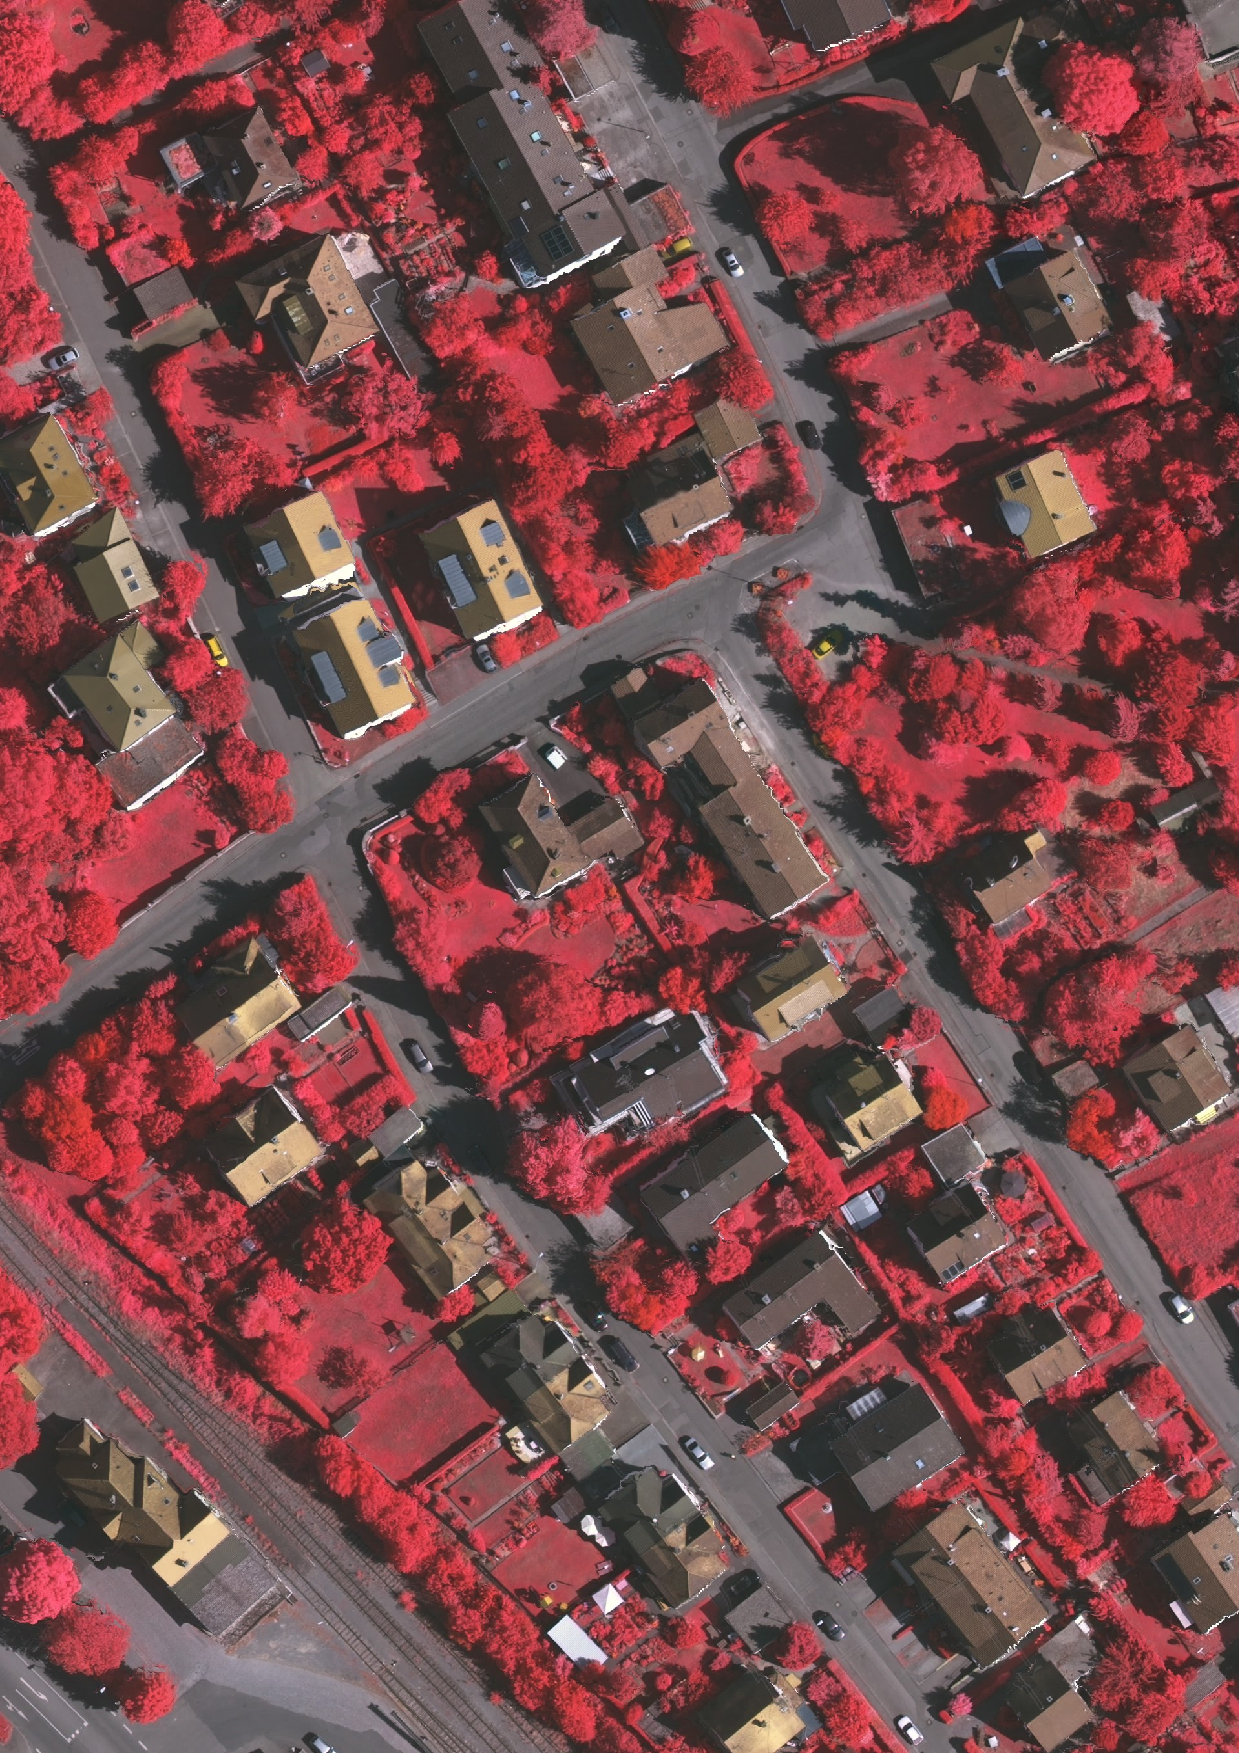
\includegraphics[width=\textwidth]{images/Image_Train.pdf}
      \caption{Train set}
      \label{fig:example_train}
  \end{subfigure}
  \hspace{0.05\textwidth}
  \begin{subfigure}[b]{0.32\textwidth}
      \centering
      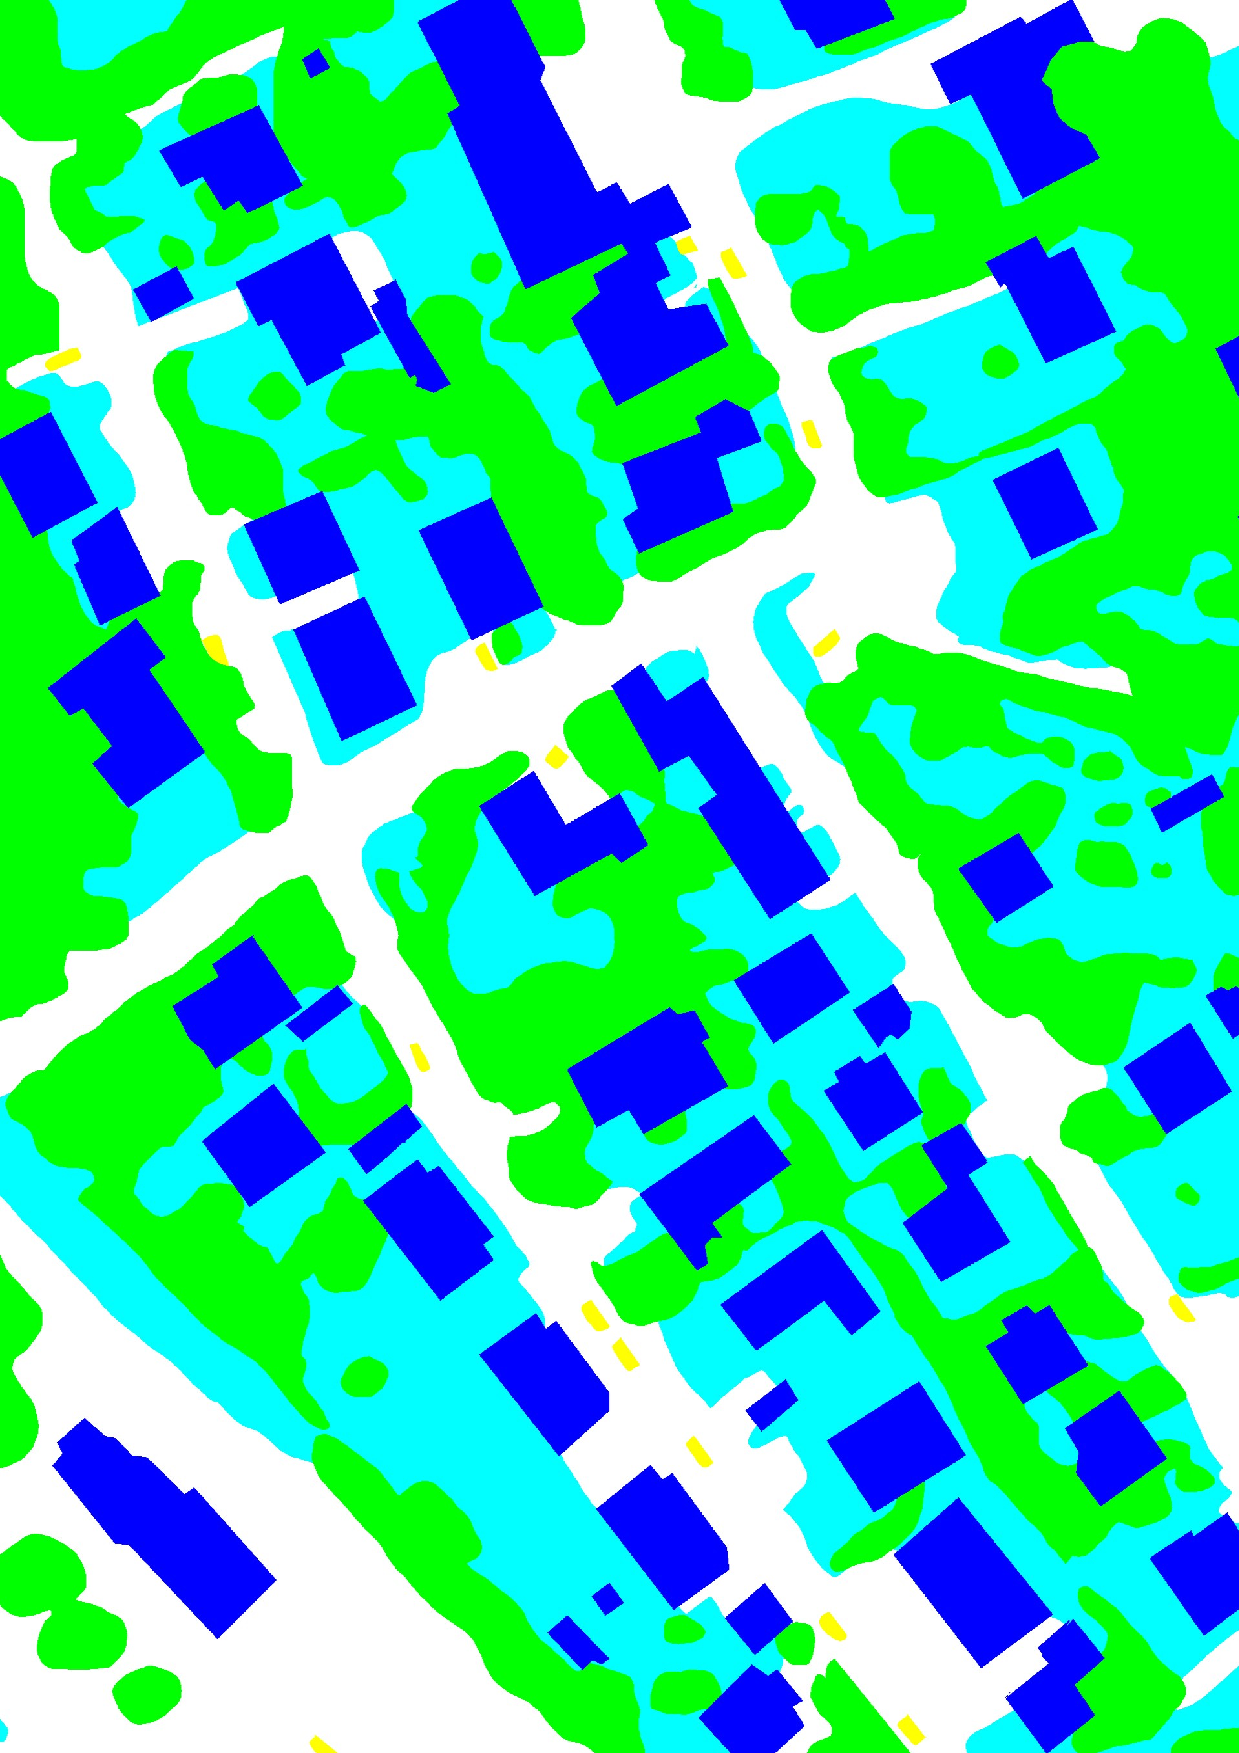
\includegraphics[width=\textwidth]{images/Reference_Train.pdf}
      \caption{Train mask}
      \label{fig:example_test}
  \end{subfigure}
  \caption{Train image to be used in the exercice}
  \label{fig:example}
\end{figure}

\subsection{Exercice}


The main objextive of this notebook is to implement a DeepLabV3+ Network for semantic segmentation using Segmentation Models of PyTorch. 
The following steps should be followed:

\begin{enumerate}
  \item Split the train image for training (80\%) and validation (20\%)
  \item Generate patches from the training image (128x128, 64x64, 32x32)
  \item Train a DeepLabV3+ network using the Segmentation Models of pytorch using the ecoder \ 
        {\tt 'mobilenet\_v2'} from scratch and with pretrained weights of {\tt 'imagenet'}, {\tt encoder\_depth = 4} \
        and {\tt decoder\_channels = [256, 128, 64, 32]}
  \item For training, use the {\tt “weighted\_categorical\_crossentropy”} as a loss function. To compute the weights you must count the number of pixels of each class
  \item Evaluate the model on the test image using patches and make the mosaic to visualize the complete image
  \item Compute metrics for each class
  \item Compare and analize the results
\end{enumerate}

Use the following mean and standard deviation values according to the adopted weights initialization:

\begin{python}
  #Normalization for ImageNet
  mean_ = [0.485, 0.456, 0.406]
  std_  = [0.229, 0.224, 0.225]

  #Normalization for trainning from scratch
  mean_ = 0.0
  std_  = 1.0
\end{python}

\subsection{Cases of study}

From the proposed exercice, the following tests will be performed and compared regardign general error metrics and confusion matrices:

\begin{enumerate}
  \item Using imagenet weights as starting values\label{item:1}
  \begin{enumerate}[a]
    \item Creating patches of 32 x 32 pixels\label{item:1a}
    \item Creating patches of 64 x 64 pixels\label{item:1b}
    \item Creating patches of 128 x 128 pixels\label{item:1c}
  \end{enumerate}
  \item Using randomly initiated weights\label{item:2}
  \begin{enumerate}[a]
    \item Creating patches of 32 x 32 pixels\label{item:2a}
    \item Creating patches of 64 x 64 pixels\label{item:2b}
    \item Creating patches of 128 x 128 pixels\label{item:2c}
  \end{enumerate}
\end{enumerate}


\section{Results and discussions}

\subsection{Colab Notebook}

All the code, examples and tests made are documented on the following Colab Notebook. 

\begin{itemize}
  \item \href{https://colab.research.google.com/drive/1CsJtybd_mc1ewyKjQQcVnqqpMvM5mJwv?usp=sharing}{Link to the Colab Notebook}
\end{itemize}

\subsection{Code Highlights}

\begin{python}
class PatchDataset(Dataset):
    
    def __init__(self, img_path, mask_path, mean, std, transform=None, n_patches=32, stride=1):
        self.img_path = img_path
        self.mask_path = mask_path
        self.transform = transform
        self.n_patches = n_patches
        self.stride = stride
        self.mean = mean
        self.std = std

        #Reading the image
        img = cv2.imread(self.img_path)
        img = cv2.cvtColor(img, cv2.COLOR_BGR2RGB)
        mask = cv2.imread(self.mask_path, cv2.IMREAD_GRAYSCALE)
        self.img = img
        self.mask = mask
        orig_gray_lbls = np.sort(np.unique(mask))
        self.label_dict = {}
        self.classes_weights = []
        class_i = 0
        for orig_lbl in orig_gray_lbls:
          mask[mask == orig_lbl] = class_i
          self.label_dict[class_i] = orig_lbl
          print(f'Total number of elements in class {class_i}: {np.sum(mask == class_i)} ({np.sum(mask == class_i)/mask.size})')
          self.classes_weights.append(mask.size/np.sum(mask == class_i))
          class_i += 1
        
        img = torch.from_numpy(img).long()
        mask = torch.from_numpy(mask).long()

        self.img_patches = img.unfold(0,self.n_patches,self.stride).unfold(1,self.n_patches,self.stride)
        self.mask_patches = mask.unfold(0,self.n_patches,self.stride).unfold(1,self.n_patches,self.stride)
        #self.img_patches = F.unfold(img,kernel_size=self.n_patches,stride=self.stride)#.unfold(1,self.n_patches,self.stride)
        #self.mask_patches = F.unfold(mask,kernel_size=self.n_patches,stride=self.stride)#.unfold(1,self.n_patches,self.stride)
        self.img_patches_shape = self.img_patches.shape
        
    def __len__(self):
        self.img_patches_shape = self.img_patches.shape
        return self.img_patches_shape[0]*self.img_patches_shape[1]
    
    def __getitem__(self, idx):

        self.img_patches_shape = self.img_patches.shape
        
        idx_x = idx % self.img_patches_shape[0]
        idx_y = idx // self.img_patches_shape[0]

        #print(idx_x, idx_y)
        img = self.img_patches[idx_x, idx_y, :, :, :]#.numpy()#.astype('int32')
        img = img.transpose(0,2).transpose(0,1).numpy().astype(np.uint8)
        #img2 = np.zeros((self.n_patches, self.n_patches, 3), dtype=np.uint8)
        #img2[:, :, 0] = img[0, :, :]
        #img2[:, :, 1] = img[1, :, :]
        #img2[:, :, 2] = img[2, :, :]

        #img = img2.copy()
        #del img2

        mask = self.mask_patches[idx_x, idx_y, :,  :].numpy()

        if self.transform is not None:
            aug = self.transform(image=img, mask=mask)
            img = Image.fromarray(aug['image'])
            mask = aug['mask']
        
        if self.transform is None:
            img = Image.fromarray(img)
        
        t = T.Compose([T.ToTensor(), T.Normalize(self.mean, self.std)])
        img = t(img)
        mask = torch.from_numpy(mask).long()
            
        return img, mask

\end{python}

\subsection{Hyperparameter selection}

\lipsum[1]

\subsection{Item \ref{item:1a}}

\lipsum[1]

\begin{figure}[htpb]
  \centering
  \begin{subfigure}[b]{0.32\textwidth}
      \centering
      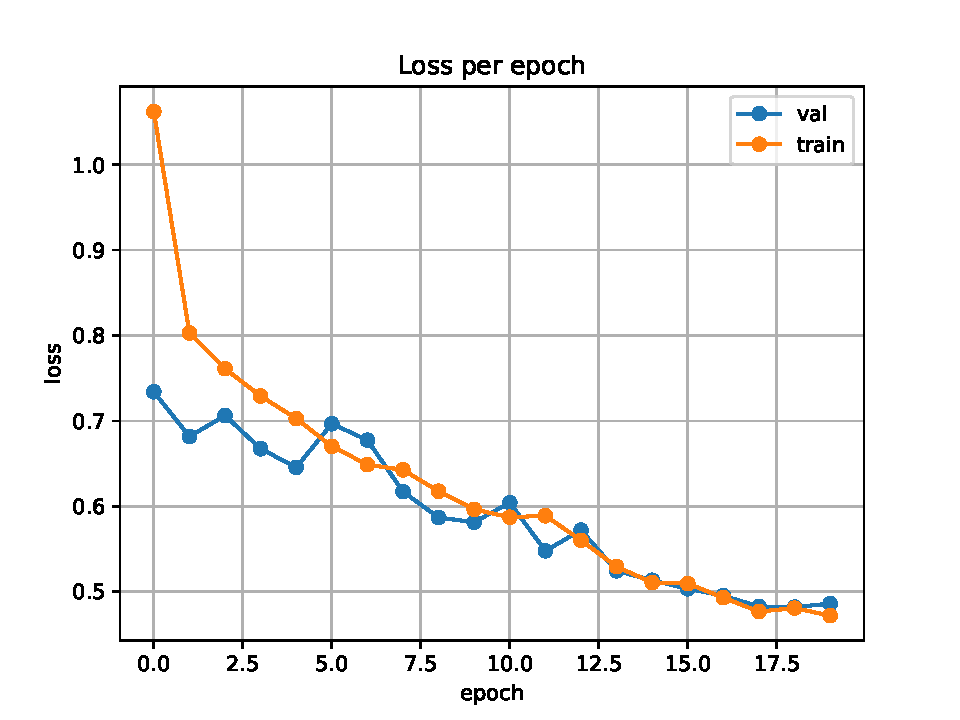
\includegraphics[width=\textwidth]{images/Patch32_imagenet_loss.pdf}
      \caption{Loss evolution}
      \label{fig:q1a_loss}
  \end{subfigure}
  \hfill
  \begin{subfigure}[b]{0.32\textwidth}
    \centering
    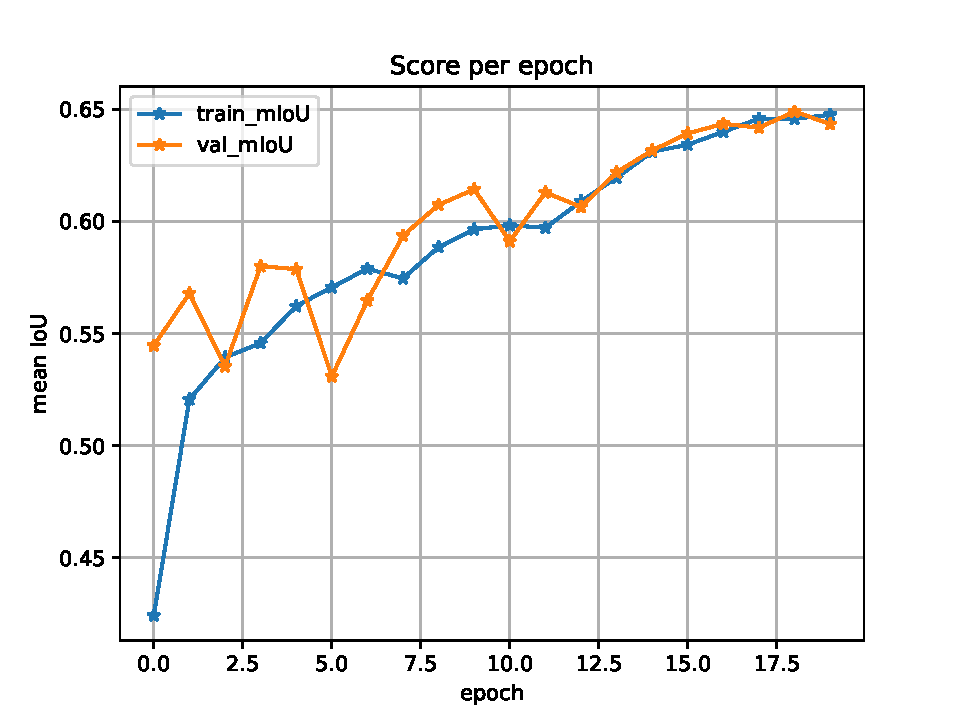
\includegraphics[width=\textwidth]{images/Patch32_imagenet_score.pdf}
    \caption{Score evolution}
    \label{fig:q1a_score}
  \end{subfigure}
  \hfill
  \begin{subfigure}[b]{0.32\textwidth}
      \centering
      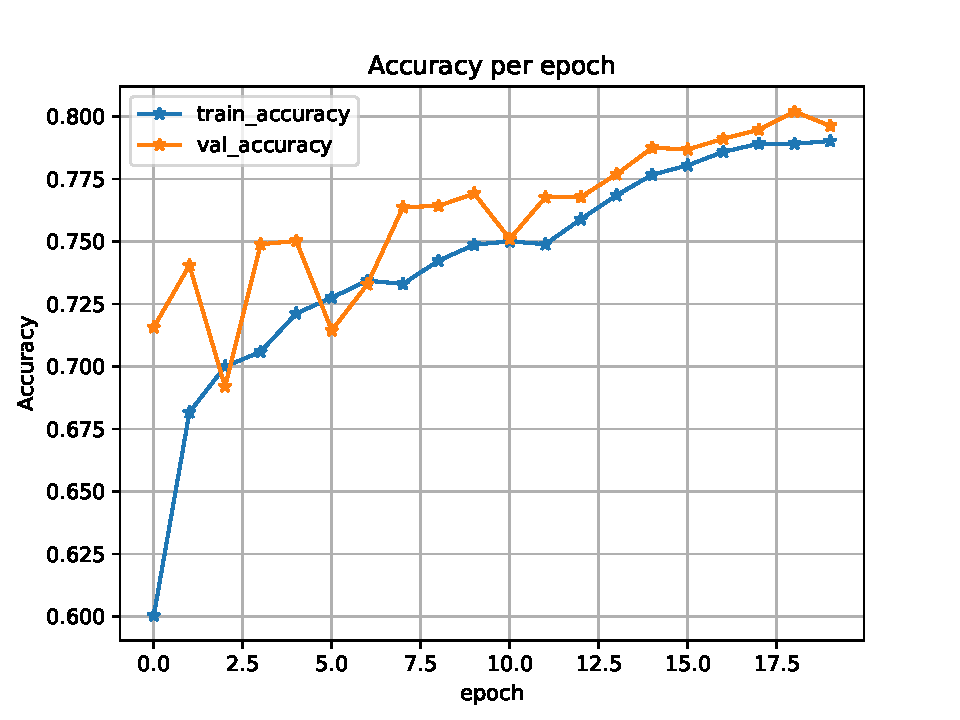
\includegraphics[width=\textwidth]{images/Patch32_imagenet_acc.pdf}
      \caption{Accuracy evolution}
      \label{fig:q1a_acc}
  \end{subfigure}
  \caption{Metrics evolution during training for item \ref{item:1a}}
  \label{fig:q1a_metrics}
\end{figure}

\begin{figure}[htpb]
  \centering
  \begin{subfigure}[b]{1.0\textwidth}
      \centering
      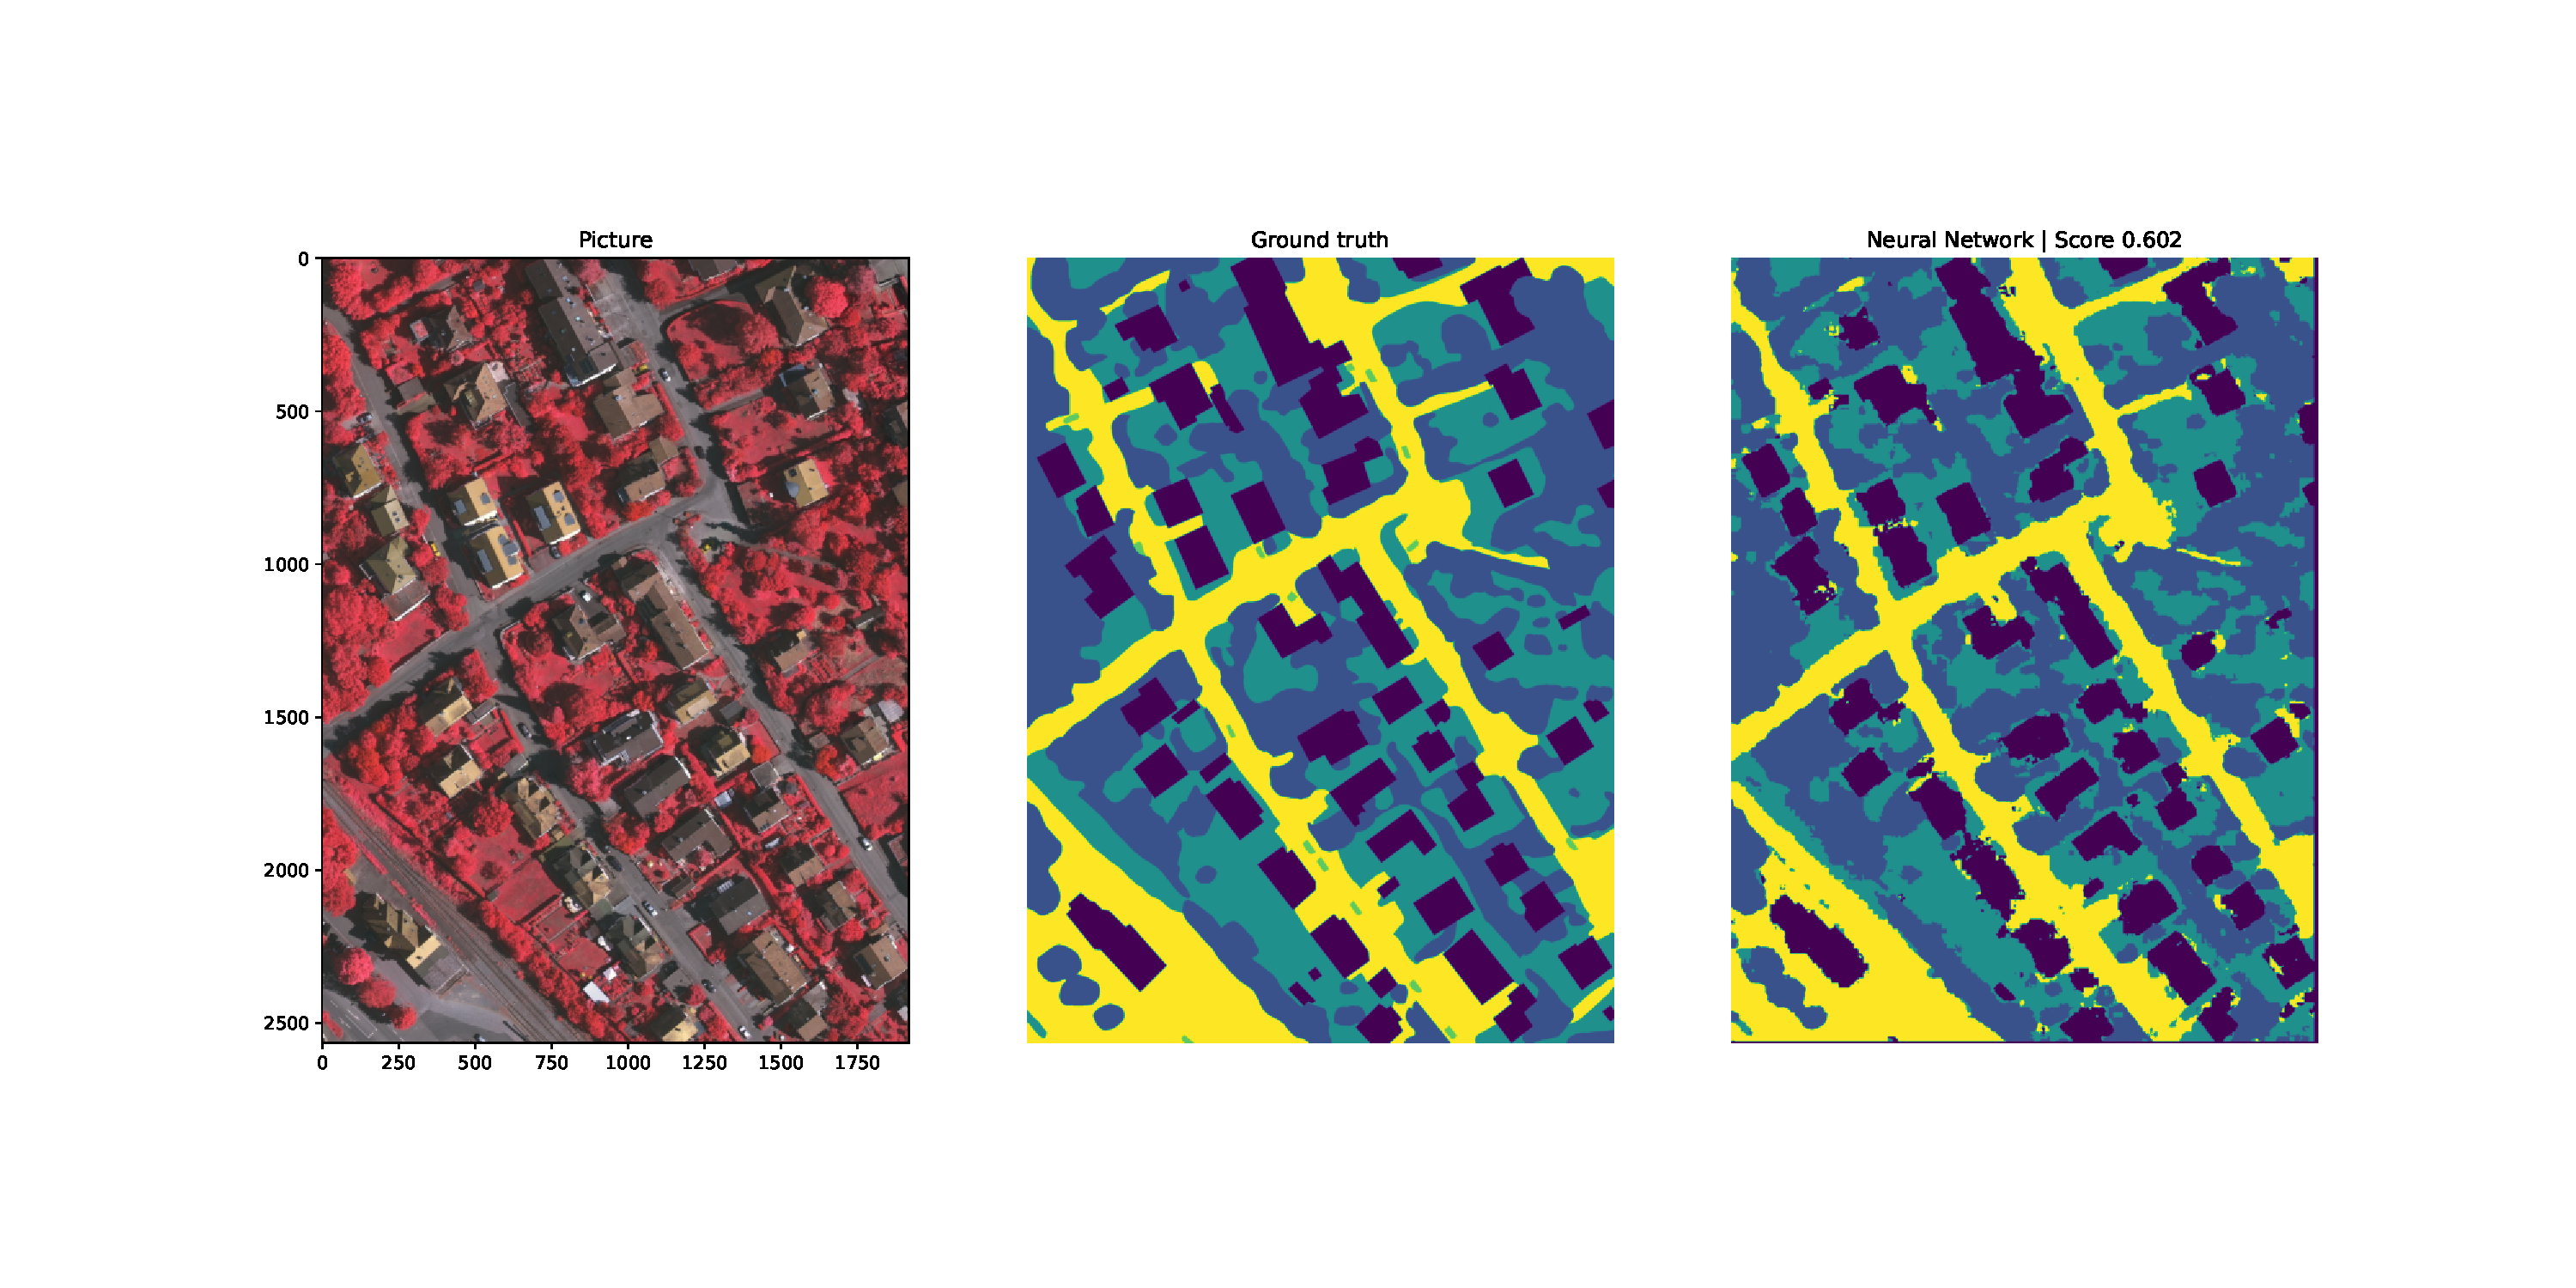
\includegraphics[width=\textwidth]{images/Patch32_imagenet_train.pdf}
      \caption{Train results}
      \label{fig:q1a_train}
  \end{subfigure}
  \hfill
  \begin{subfigure}[b]{1.0\textwidth}
    \centering
    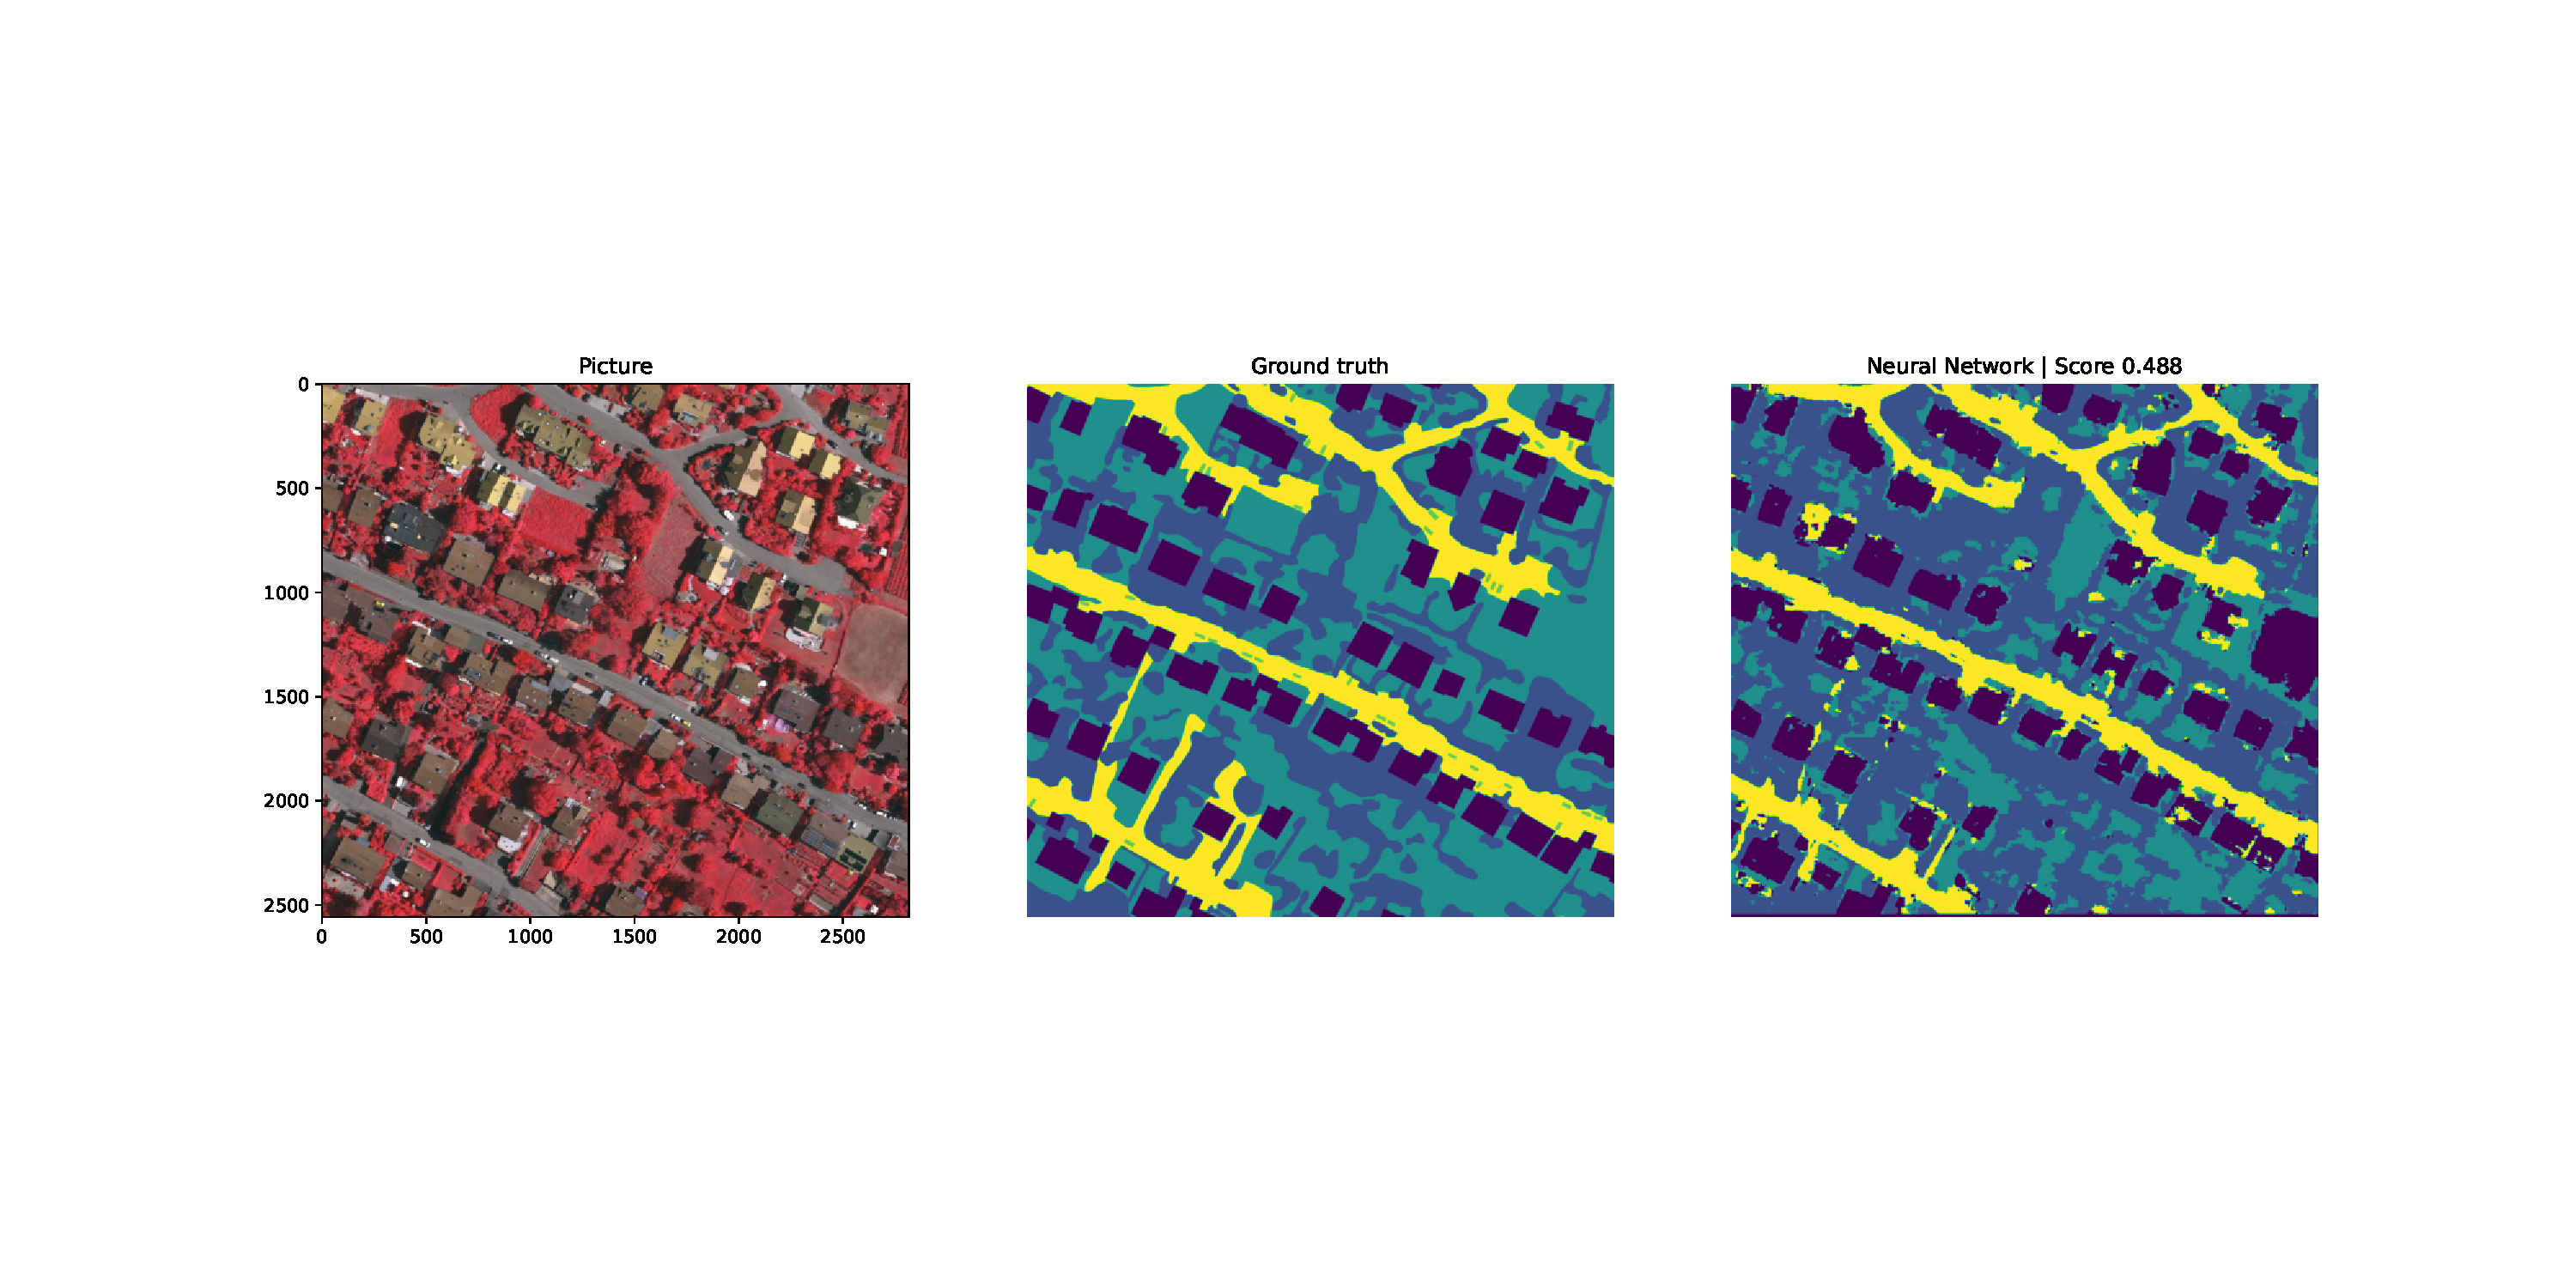
\includegraphics[width=\textwidth]{images/Patch32_imagenet_test.pdf}
    \caption{test results}
    \label{fig:q1a_test}
  \end{subfigure}
  \caption{Results of predictions for item \ref{item:1a}}
  \label{fig:q1a_results}
\end{figure}

\subsection{Item \ref{item:1b}}

\lipsum[1]

\begin{figure}[htpb]
  \centering
  \begin{subfigure}[b]{0.32\textwidth}
      \centering
      
\includegraphics[width=\textwidth]{images/Patch64_imagenet_loss.pdf}
      \caption{Loss evolution}
      \label{fig:q1b_loss}
  \end{subfigure}
  \hfill
  \begin{subfigure}[b]{0.32\textwidth}
    \centering
    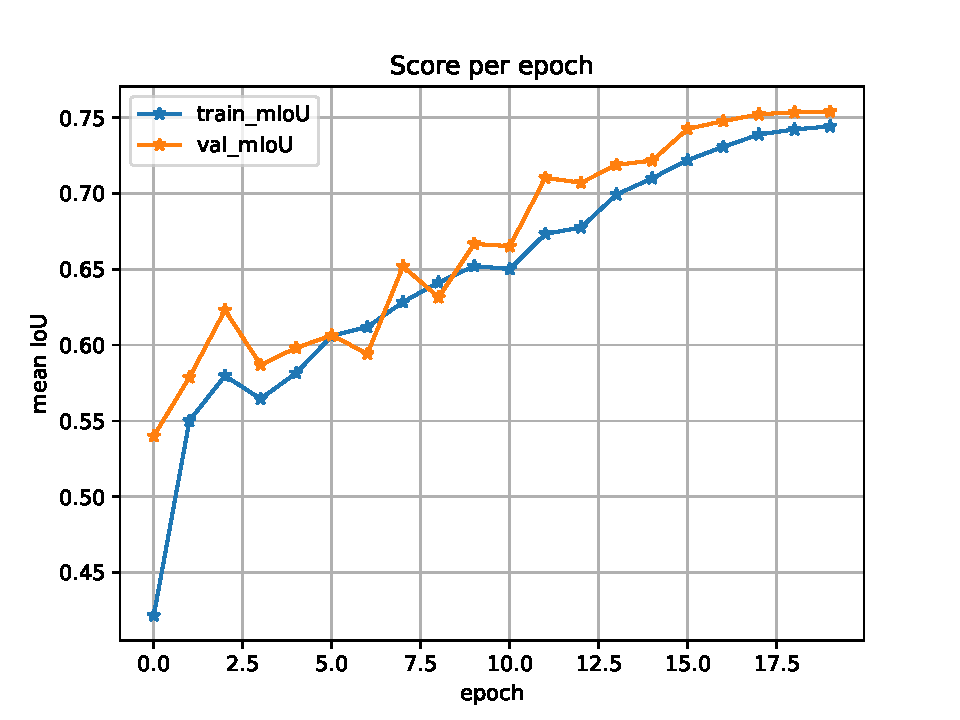
\includegraphics[width=\textwidth]{images/Patch64_imagenet_score.pdf}
    \caption{Score evolution}
    \label{fig:q1b_score}
  \end{subfigure}
  \hfill
  \begin{subfigure}[b]{0.32\textwidth}
      \centering
      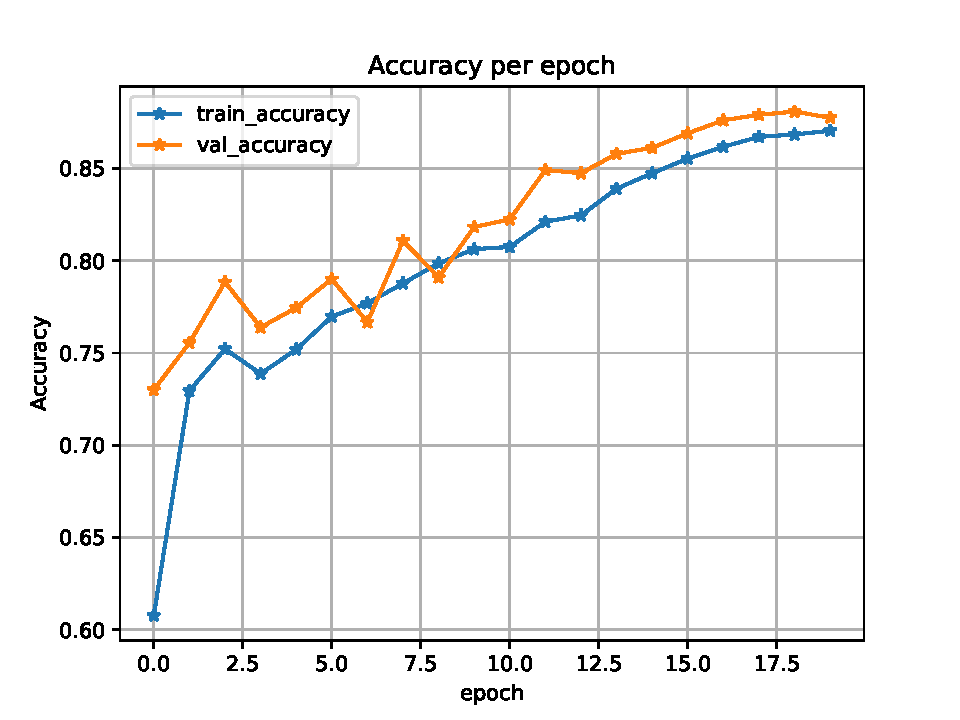
\includegraphics[width=\textwidth]{images/Patch64_imagenet_acc.pdf}
      \caption{Accuracy evolution}
      \label{fig:q1b_acc}
  \end{subfigure}
  \caption{Metrics evolution during training for item \ref{item:1b}}
  \label{fig:q1b_metrics}
\end{figure}

\begin{figure}[htpb]
  \centering
  \begin{subfigure}[b]{1.0\textwidth}
      \centering
      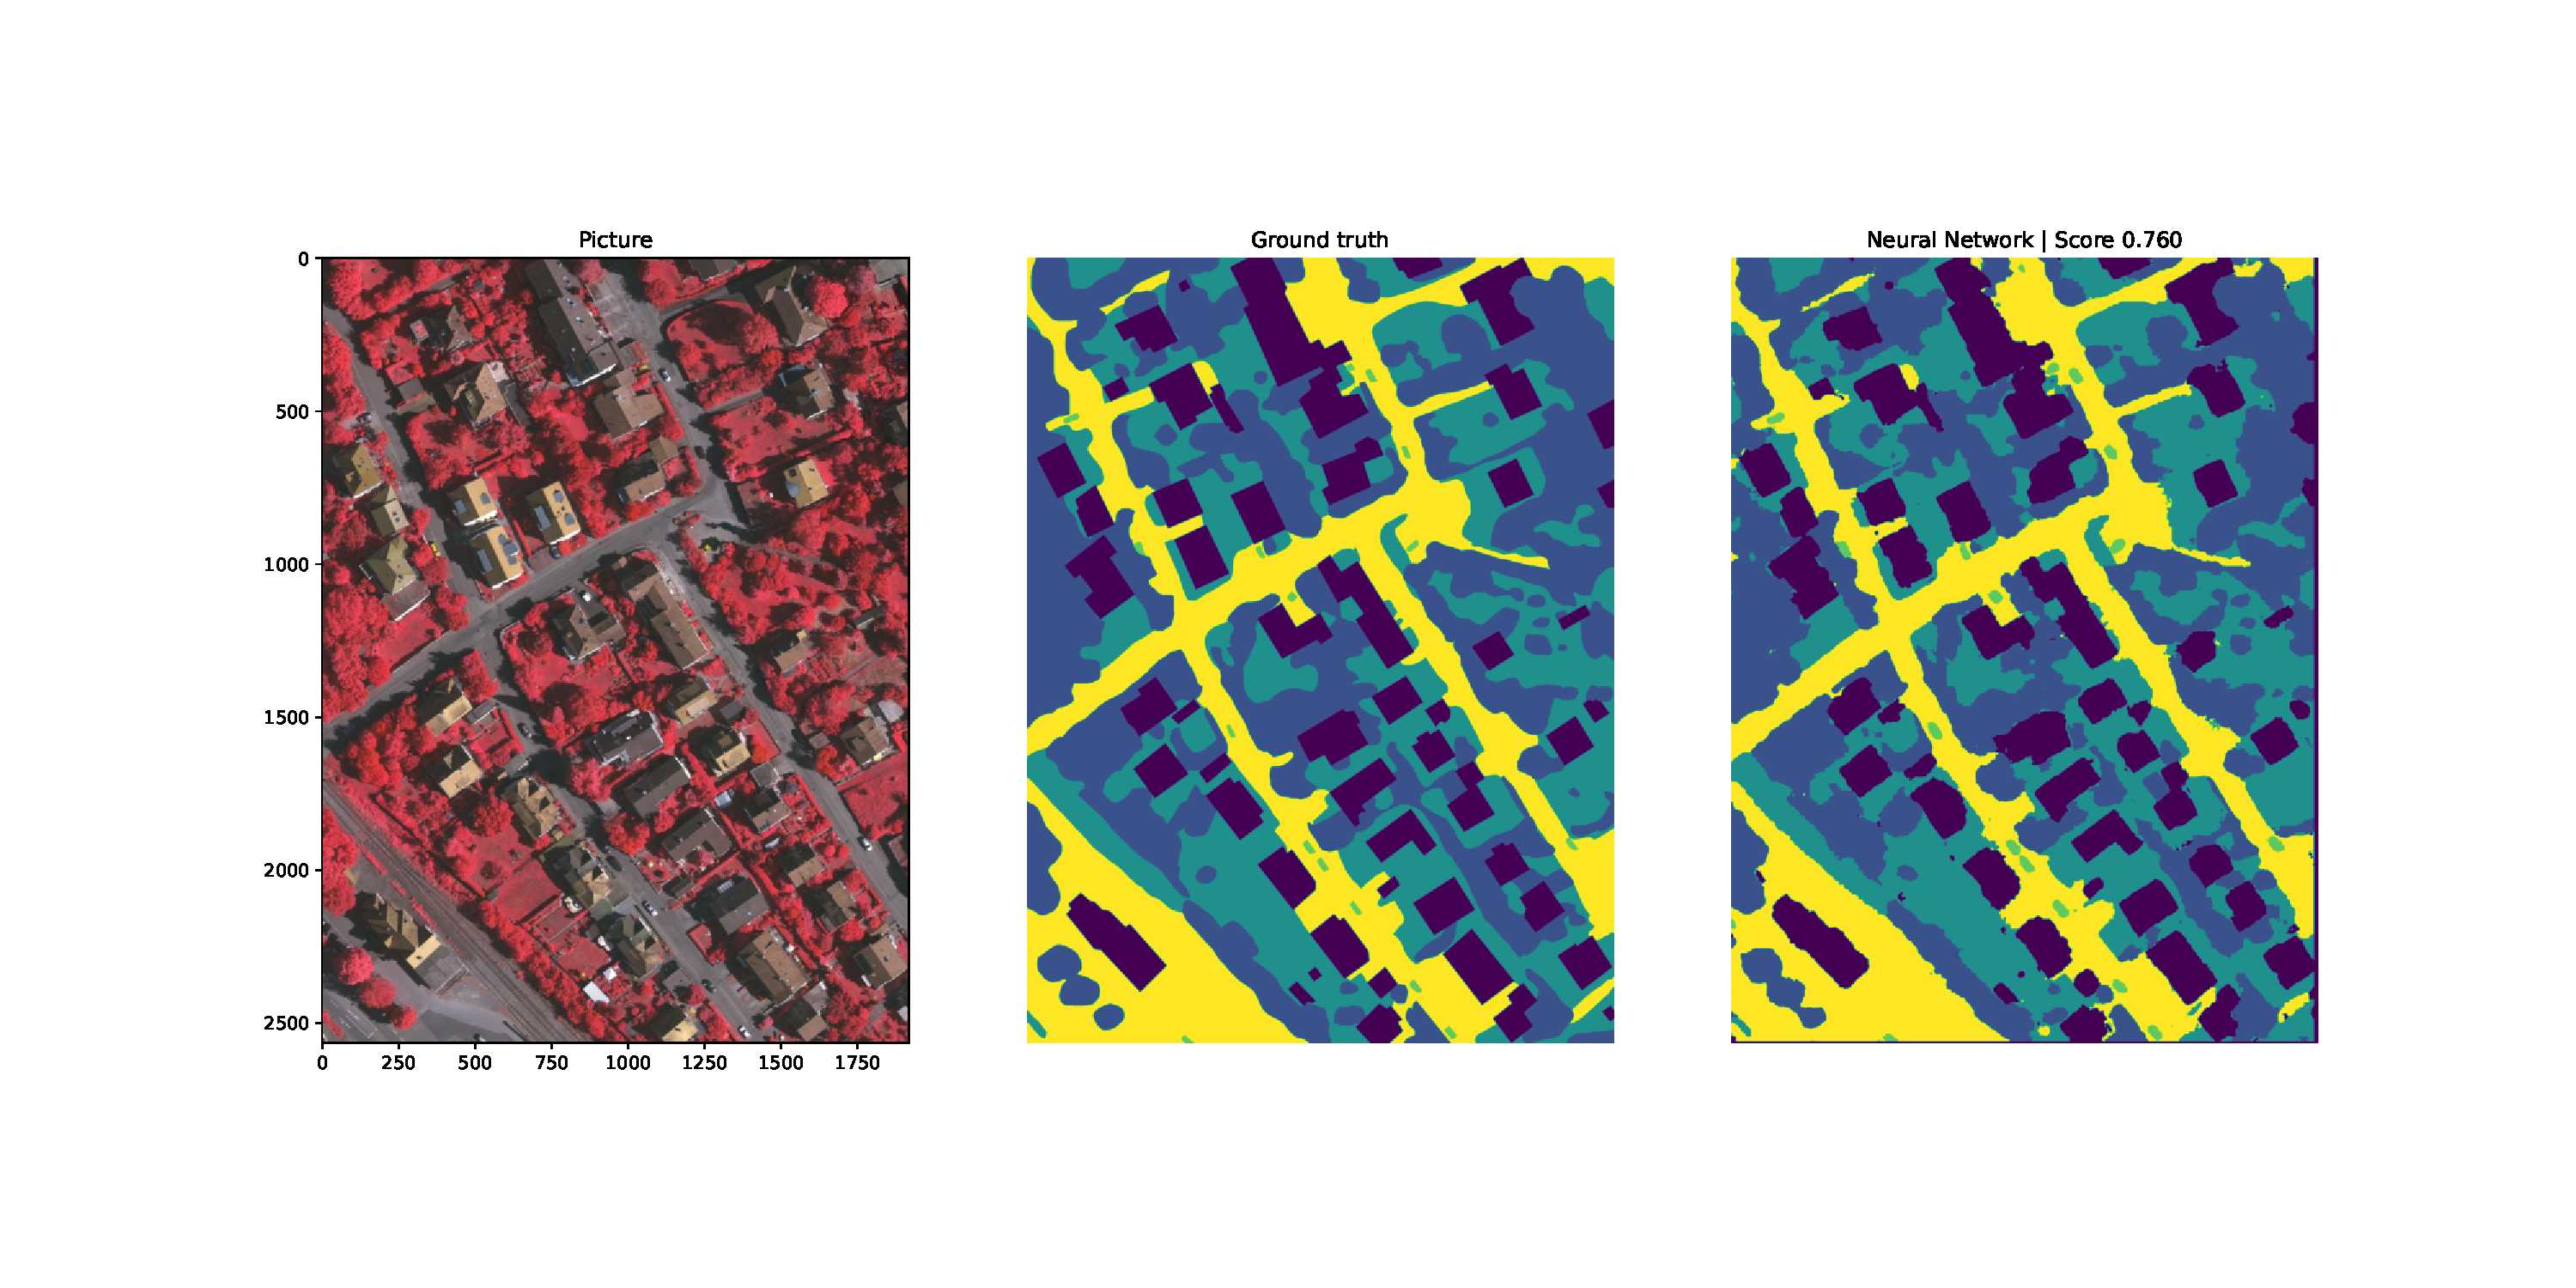
\includegraphics[width=\textwidth]{images/Patch64_imagenet_train.pdf}
      \caption{Train results}
      \label{fig:q1b_train}
  \end{subfigure}
  \hfill
  \begin{subfigure}[b]{1.0\textwidth}
    \centering
    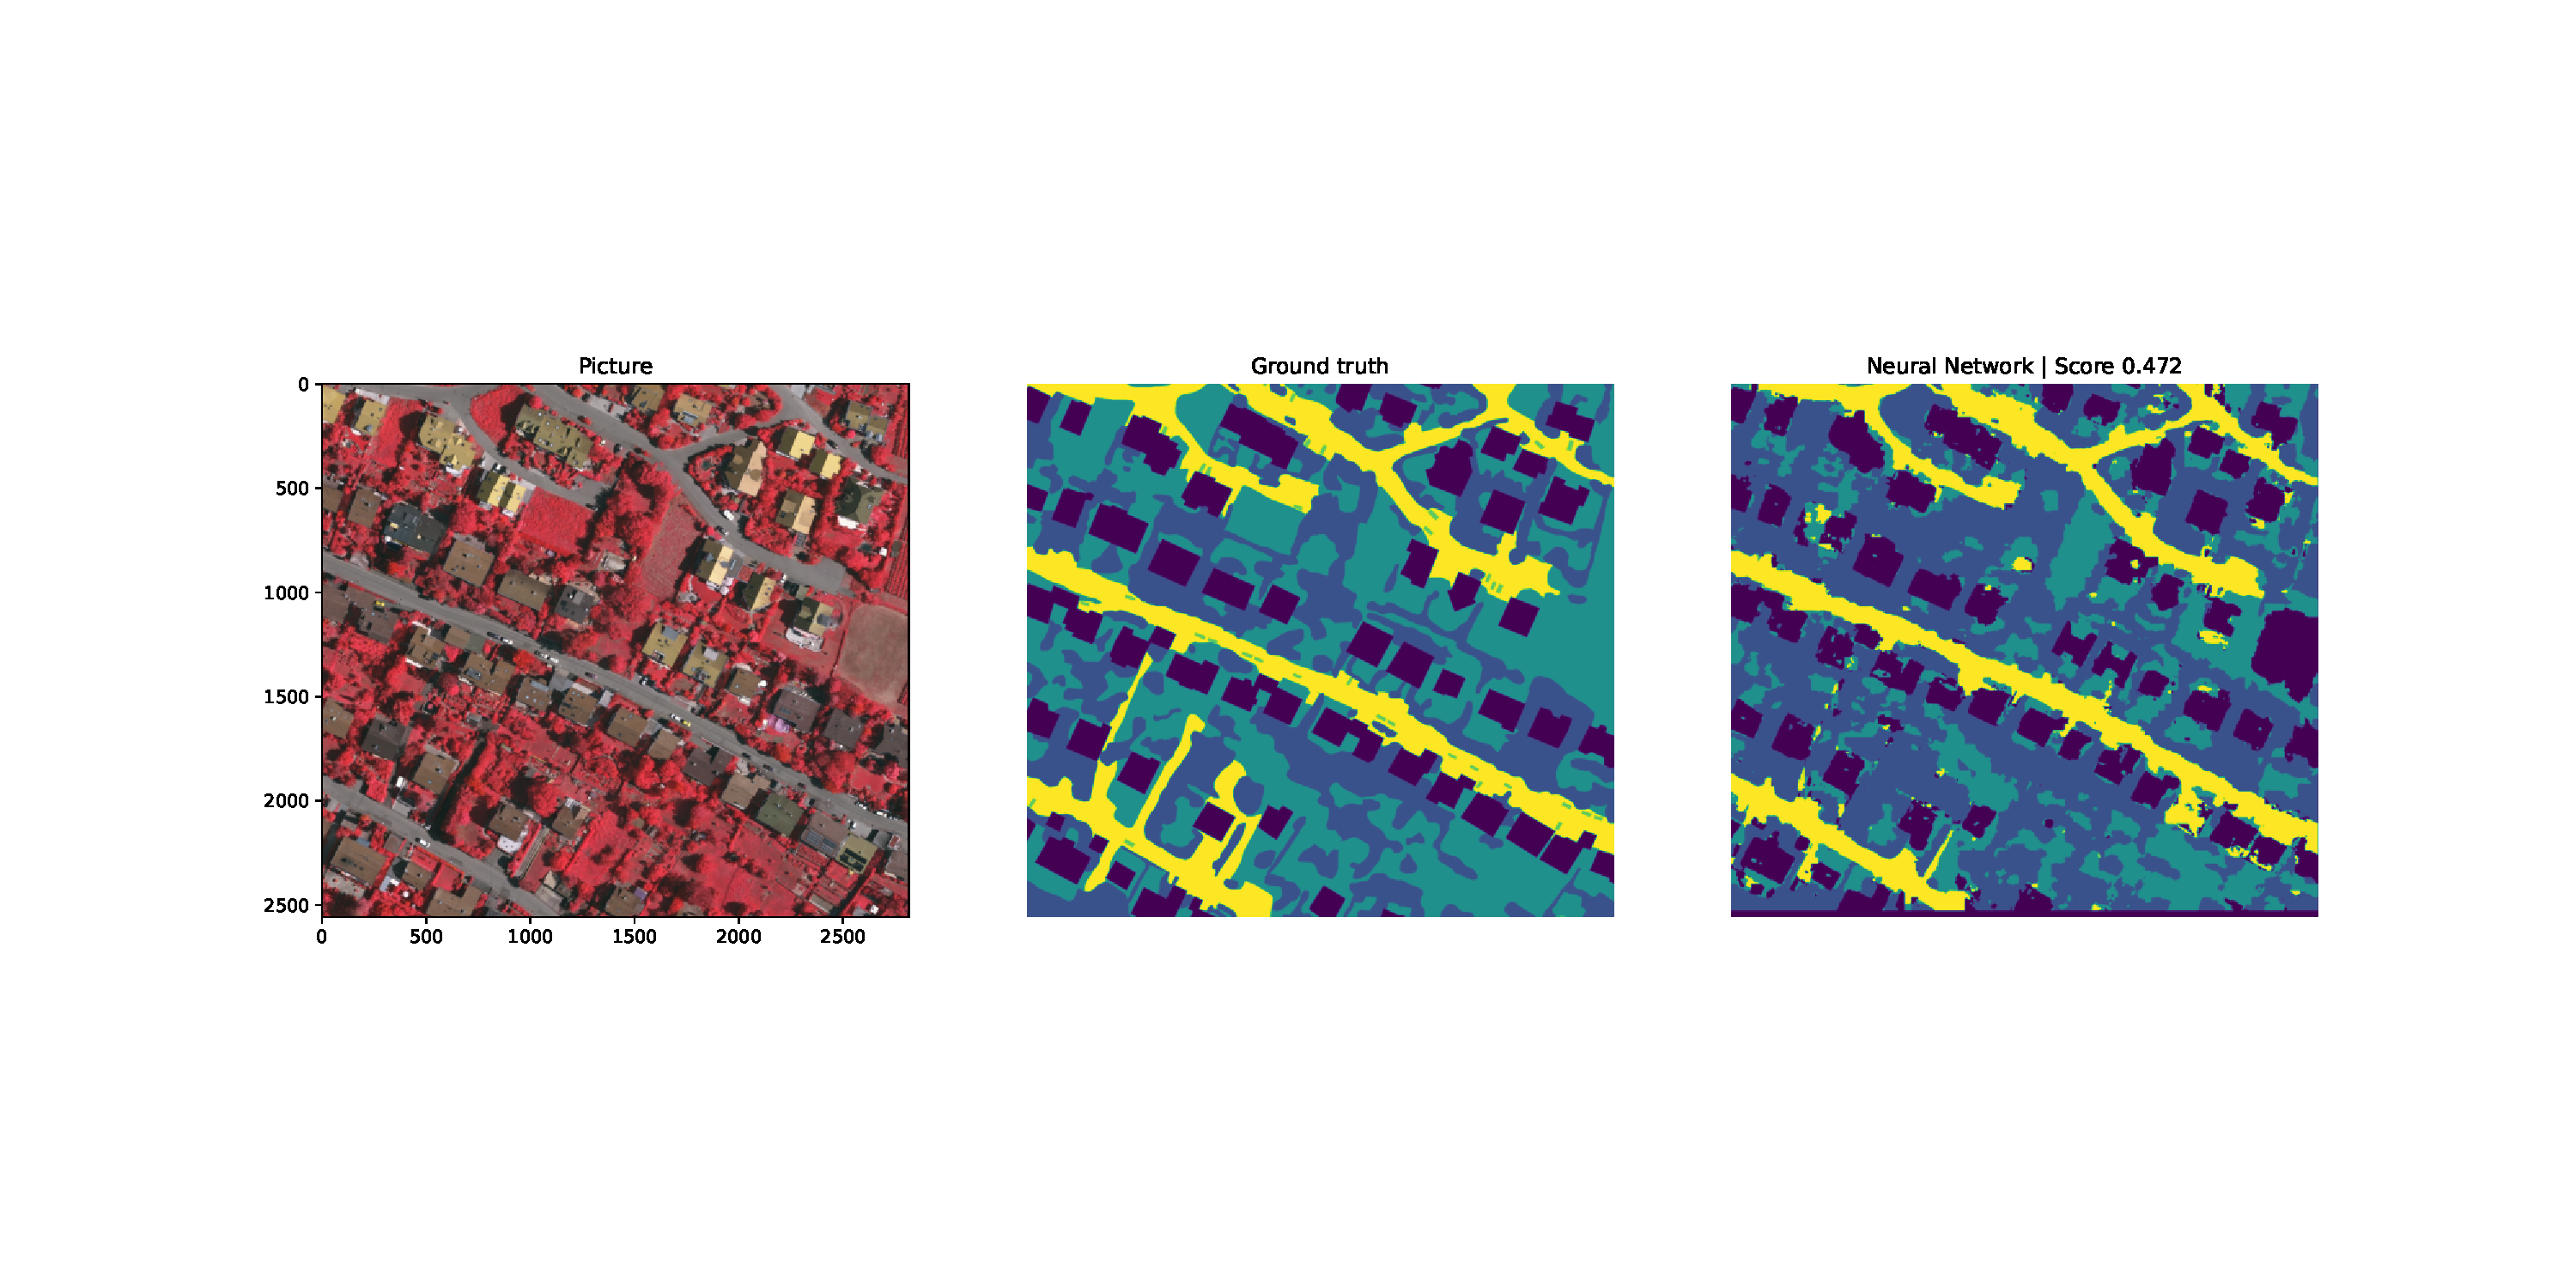
\includegraphics[width=\textwidth]{images/Patch64_imagenet_test.pdf}
    \caption{test results}
    \label{fig:q1b_test}
  \end{subfigure}
  \caption{Results of predictions for item \ref{item:1b}}
  \label{fig:q1b_results}
\end{figure}

\subsection{Item \ref{item:1c}}

\lipsum[1]

\begin{figure}[htpb]
  \centering
  \begin{subfigure}[b]{0.32\textwidth}
      \centering
      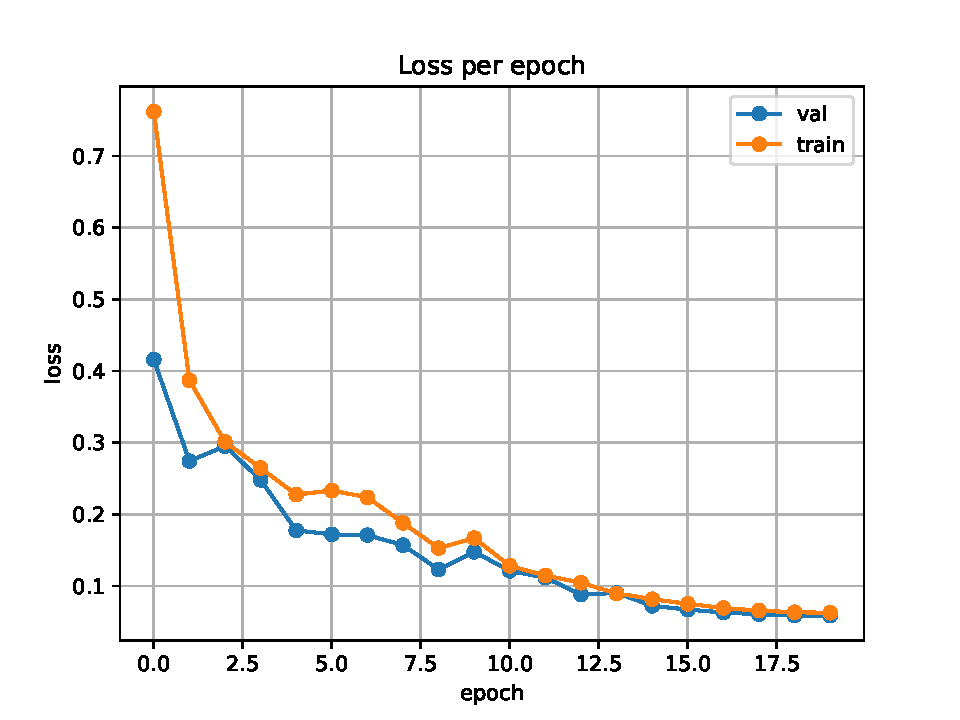
\includegraphics[width=\textwidth]{images/Patch128_imagenet_loss.pdf}
      \caption{Loss evolution}
      \label{fig:q1c_loss}
  \end{subfigure}
  \hfill
  \begin{subfigure}[b]{0.32\textwidth}
    \centering
    
\includegraphics[width=\textwidth]{images/Patch128_imagenet_score.pdf}
    \caption{Score evolution}
    \label{fig:q1c_score}
  \end{subfigure}
  \hfill
  \begin{subfigure}[b]{0.32\textwidth}
      \centering
      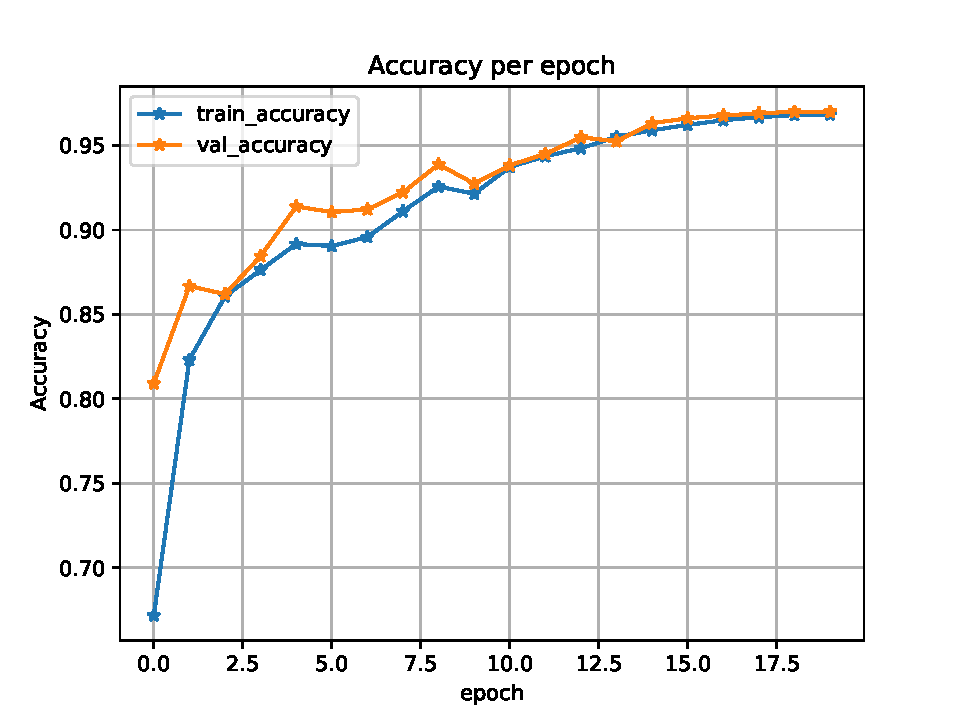
\includegraphics[width=\textwidth]{images/Patch128_imagenet_acc.pdf}
      \caption{Accuracy evolution}
      \label{fig:q1c_acc}
  \end{subfigure}
  \caption{Metrics evolution during training for item \ref{item:1c}}
  \label{fig:q1c_metrics}
\end{figure}

\begin{figure}[htpb]
  \centering
  \begin{subfigure}[b]{1.0\textwidth}
      \centering
      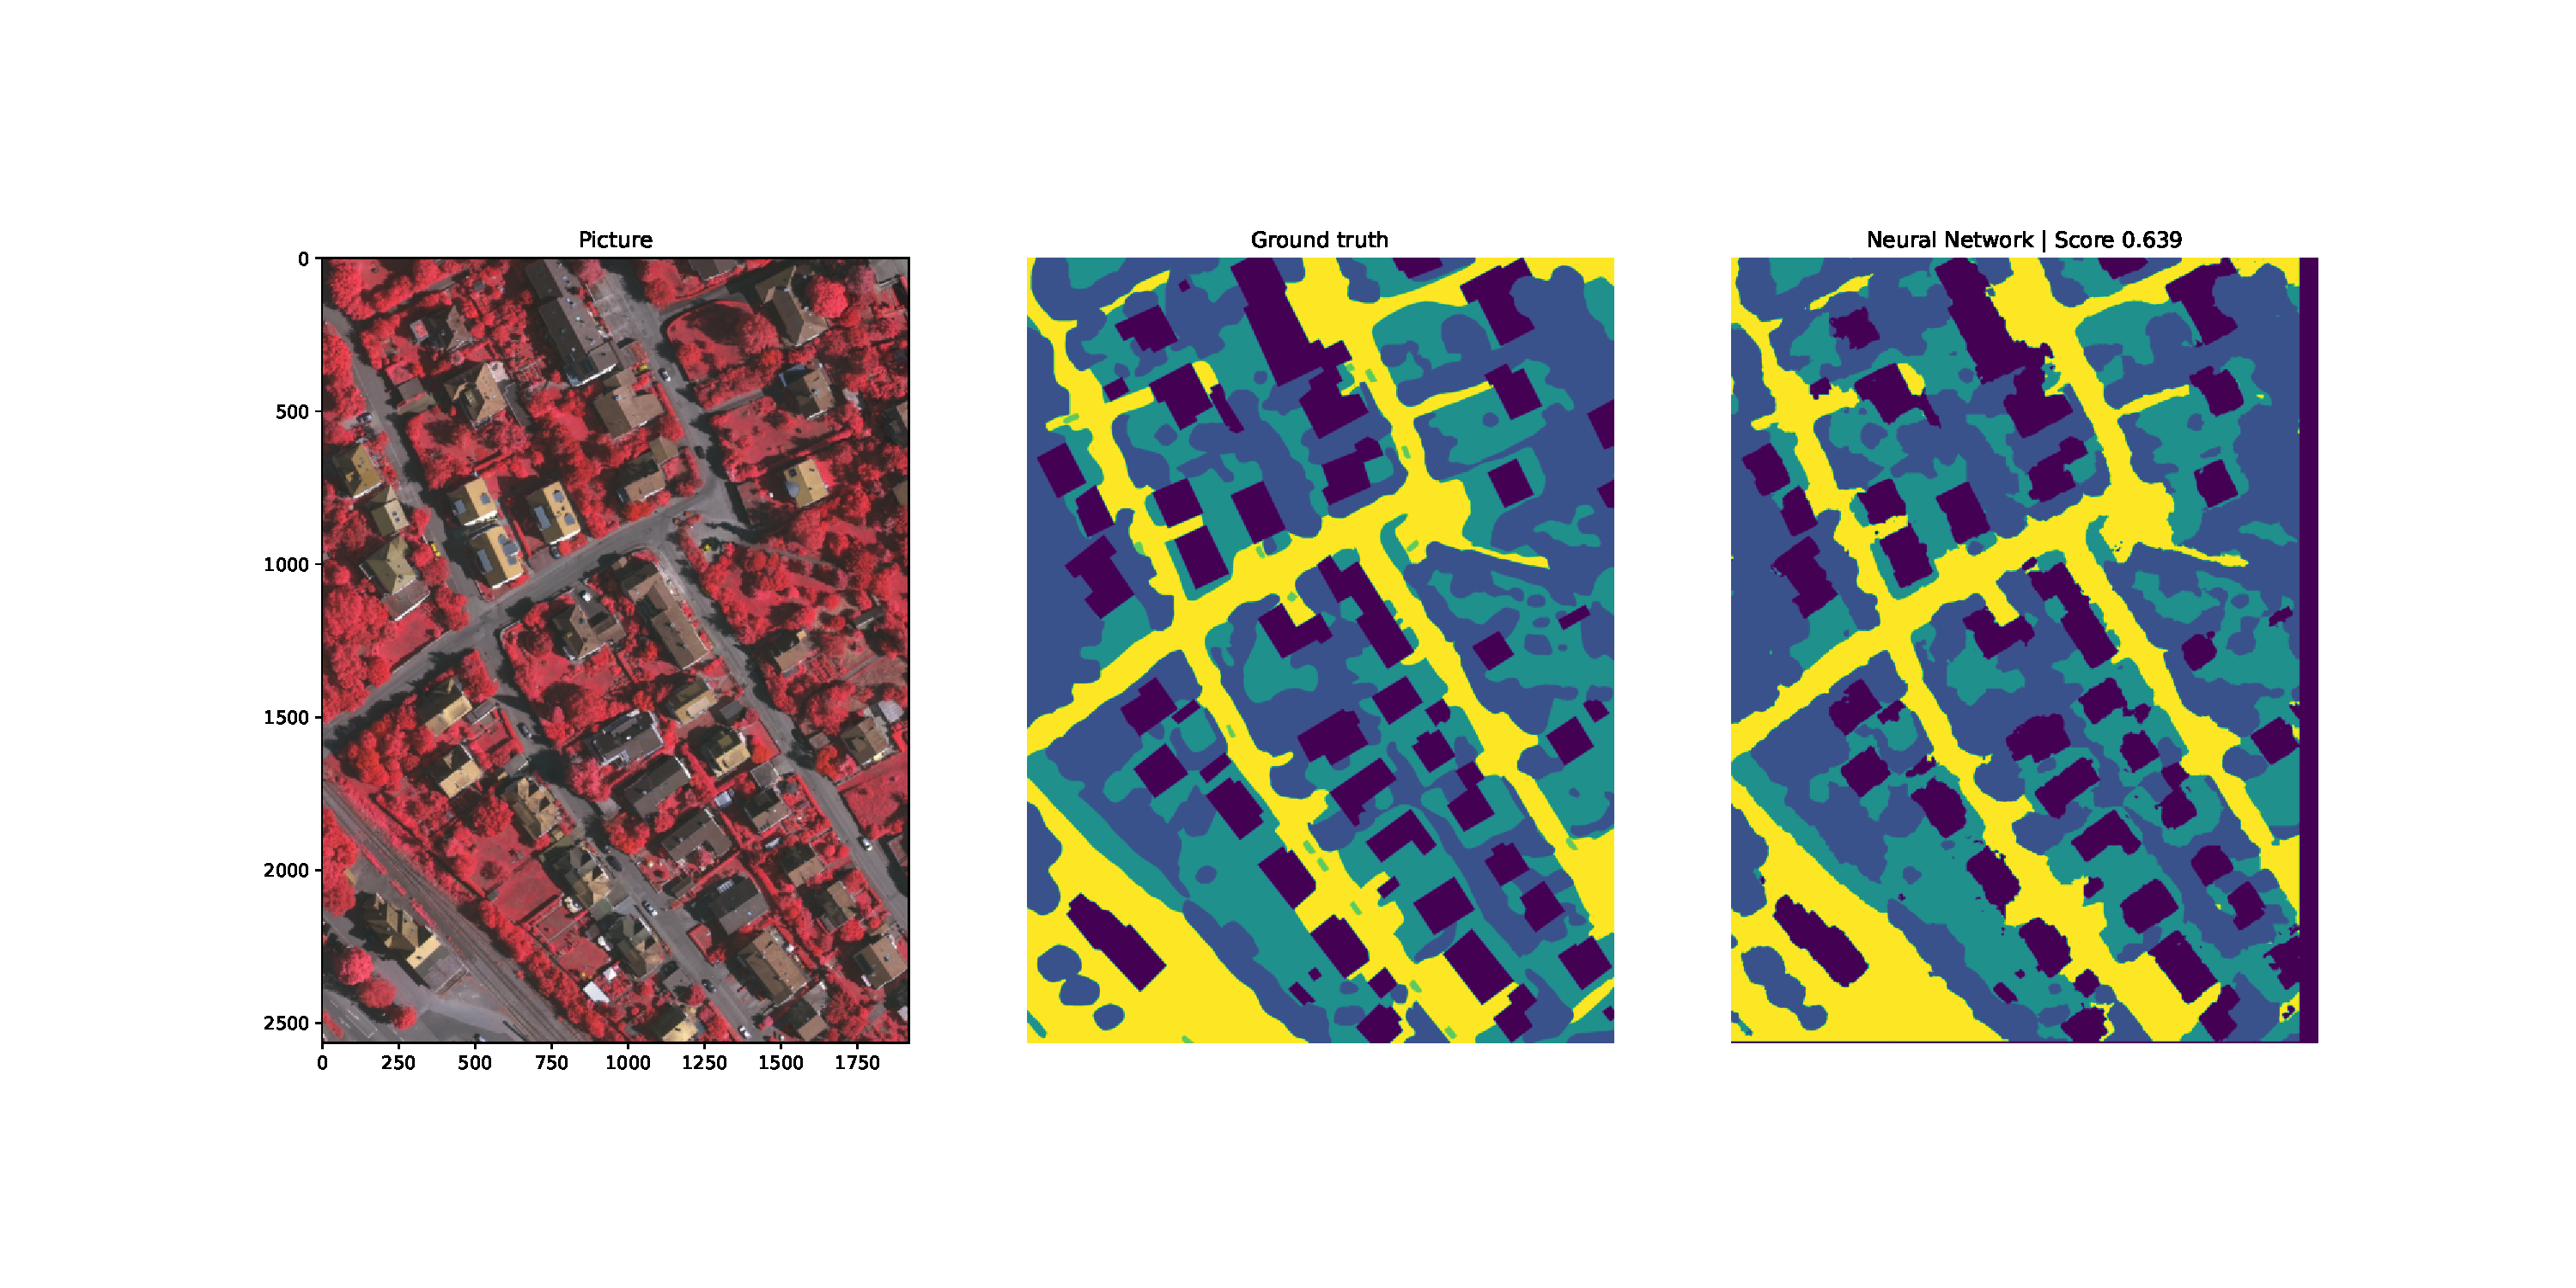
\includegraphics[width=\textwidth]{images/Patch128_imagenet_train.pdf}
      \caption{Train results}
      \label{fig:q1c_train}
  \end{subfigure}
  \hfill
  \begin{subfigure}[b]{1.0\textwidth}
    \centering
    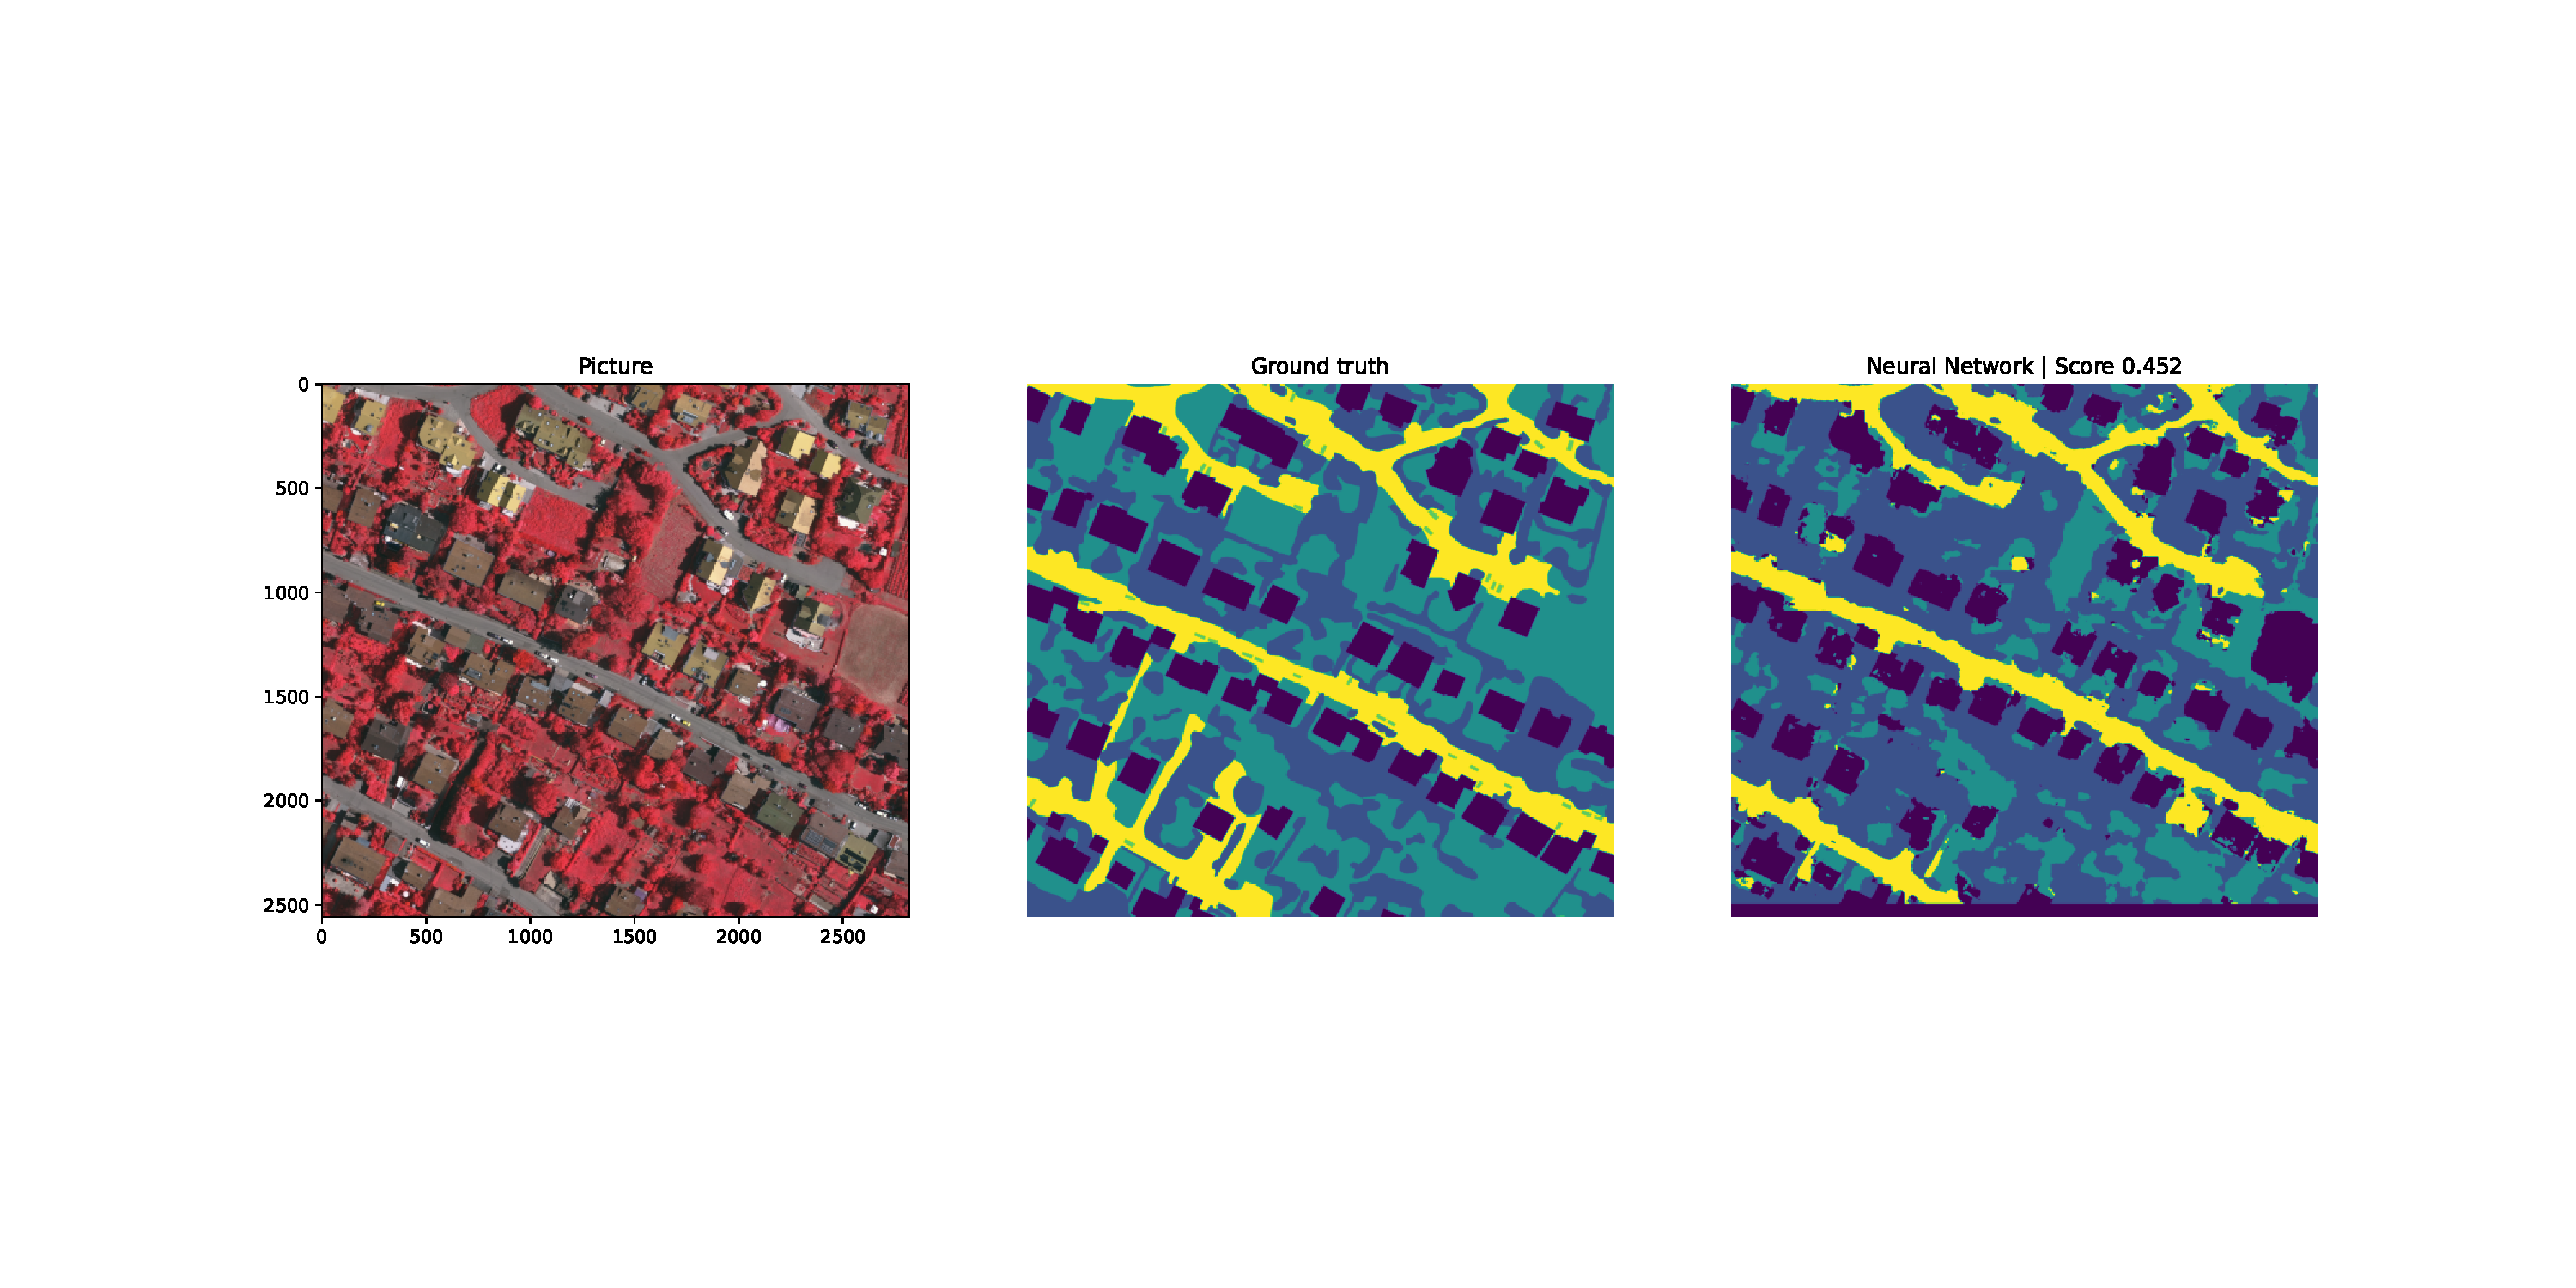
\includegraphics[width=\textwidth]{images/Patch128_imagenet_test.pdf}
    \caption{test results}
    \label{fig:q1c_test}
  \end{subfigure}
  \caption{Results of predictions for item \ref{item:1c}}
  \label{fig:q1c_results}
\end{figure}

\subsection{Item \ref{item:2a}}

\lipsum[1]

\begin{figure}[htpb]
  \centering
  \begin{subfigure}[b]{0.32\textwidth}
      \centering
      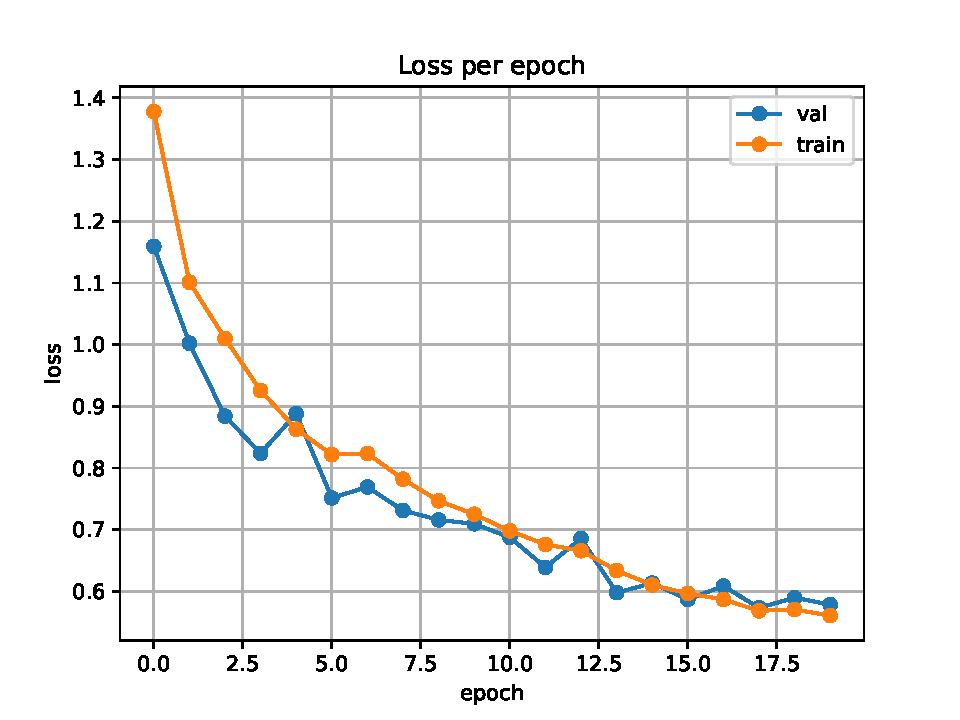
\includegraphics[width=\textwidth]{images/Patch32_scratch_loss.pdf}
      \caption{Loss evolution}
      \label{fig:q2a_loss}
  \end{subfigure}
  \hfill
  \begin{subfigure}[b]{0.32\textwidth}
    \centering
    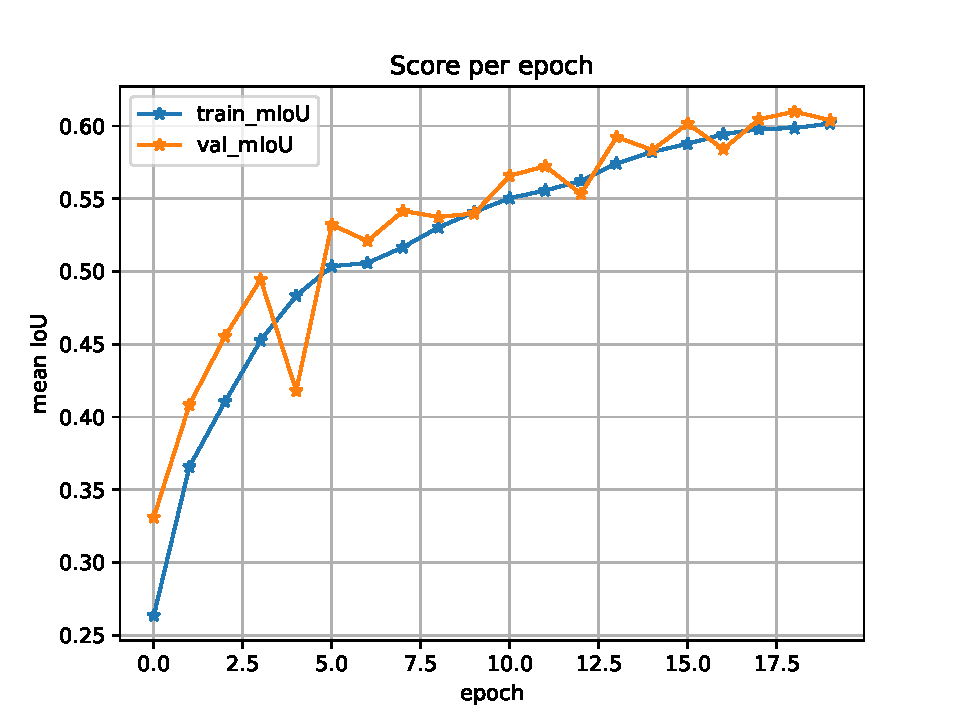
\includegraphics[width=\textwidth]{images/Patch32_scratch_score.pdf}
    \caption{Score evolution}
    \label{fig:q2a_score}
  \end{subfigure}
  \hfill
  \begin{subfigure}[b]{0.32\textwidth}
      \centering
      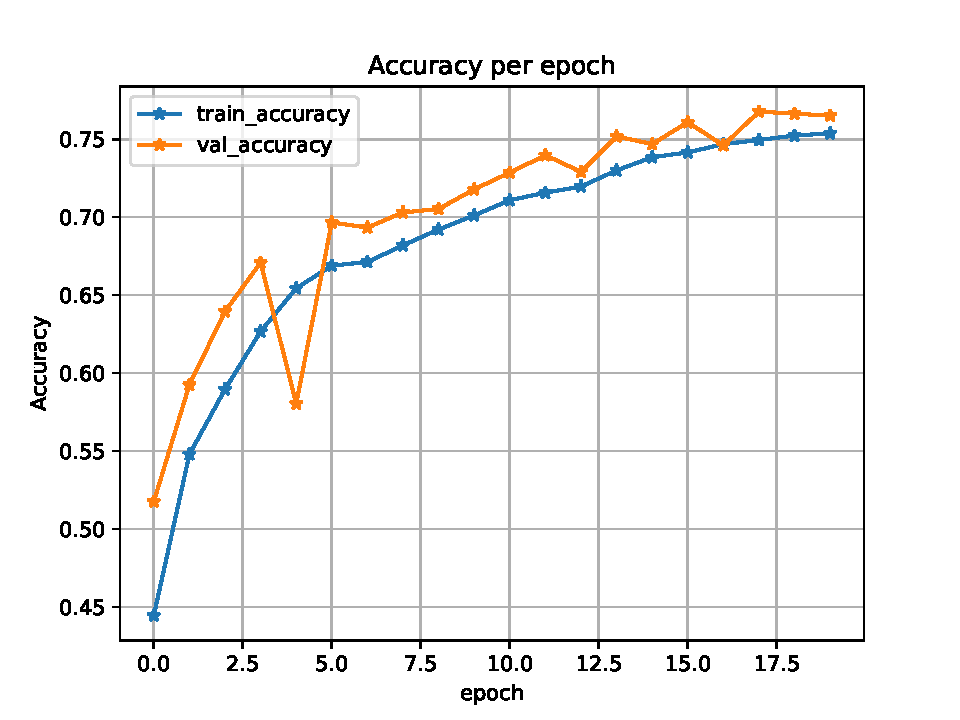
\includegraphics[width=\textwidth]{images/Patch32_scratch_acc.pdf}
      \caption{Accuracy evolution}
      \label{fig:q2a_acc}
  \end{subfigure}
  \caption{Metrics evolution during training for item \ref{item:2a}}
  \label{fig:q2a_metrics}
\end{figure}

\begin{figure}[htpb]
  \centering
  \begin{subfigure}[b]{1.0\textwidth}
      \centering
      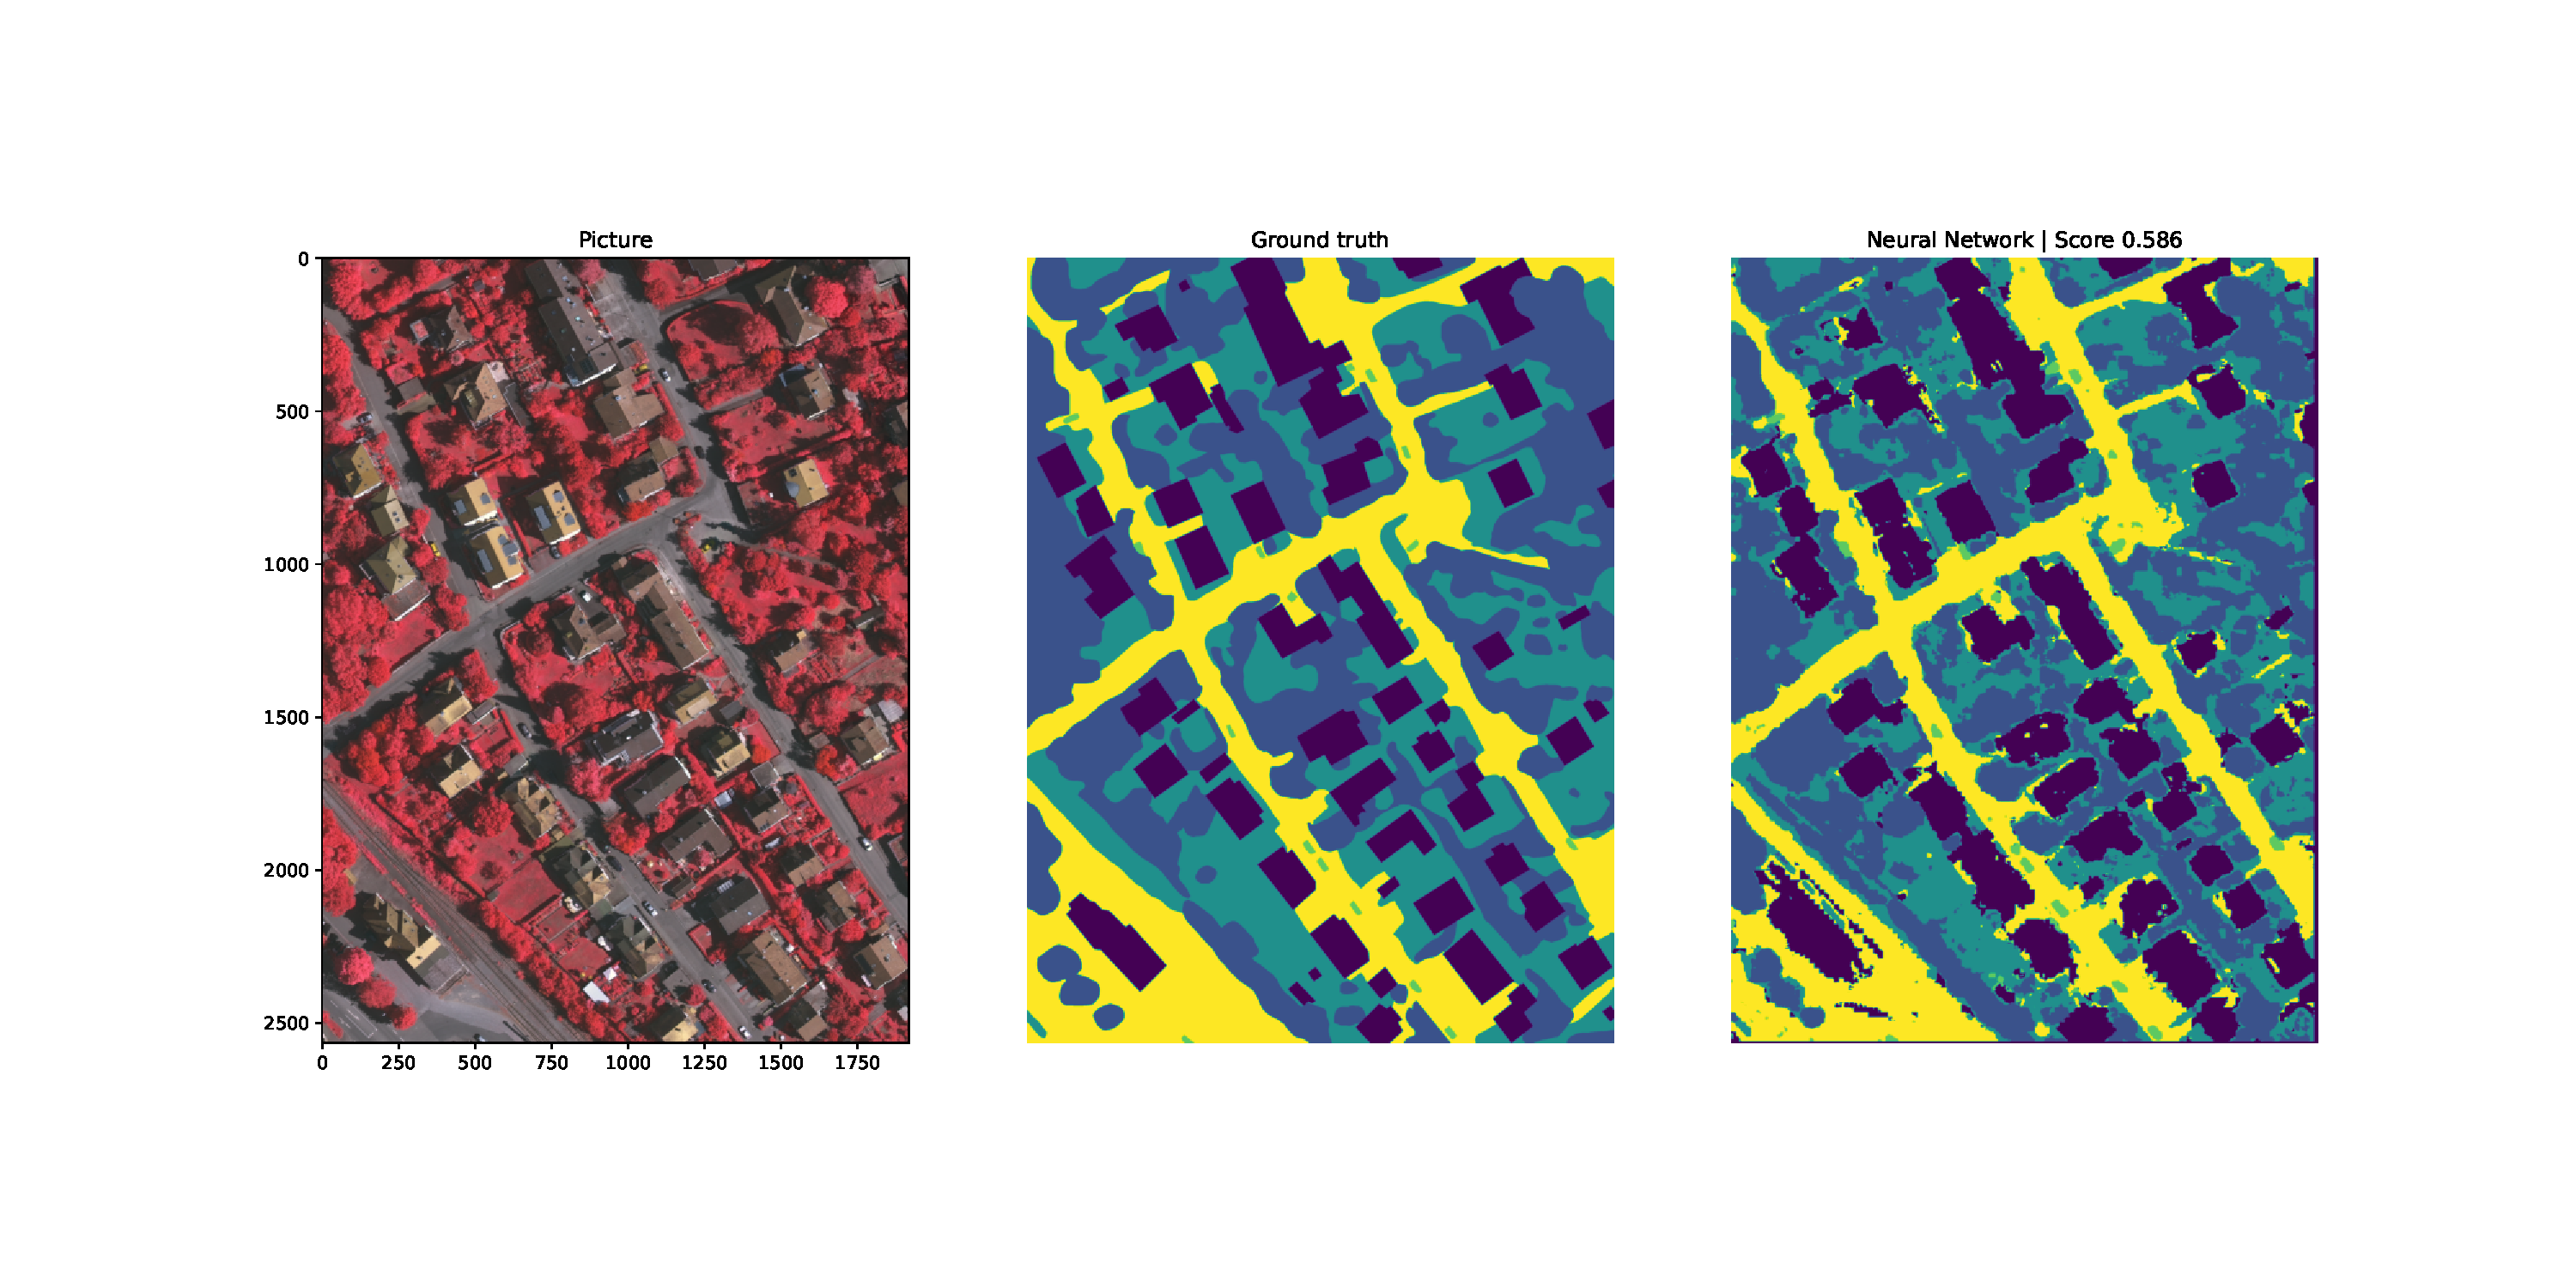
\includegraphics[width=\textwidth]{images/Patch32_scratch_train.pdf}
      \caption{Train results}
      \label{fig:q2a_train}
  \end{subfigure}
  \hfill
  \begin{subfigure}[b]{1.0\textwidth}
    \centering
    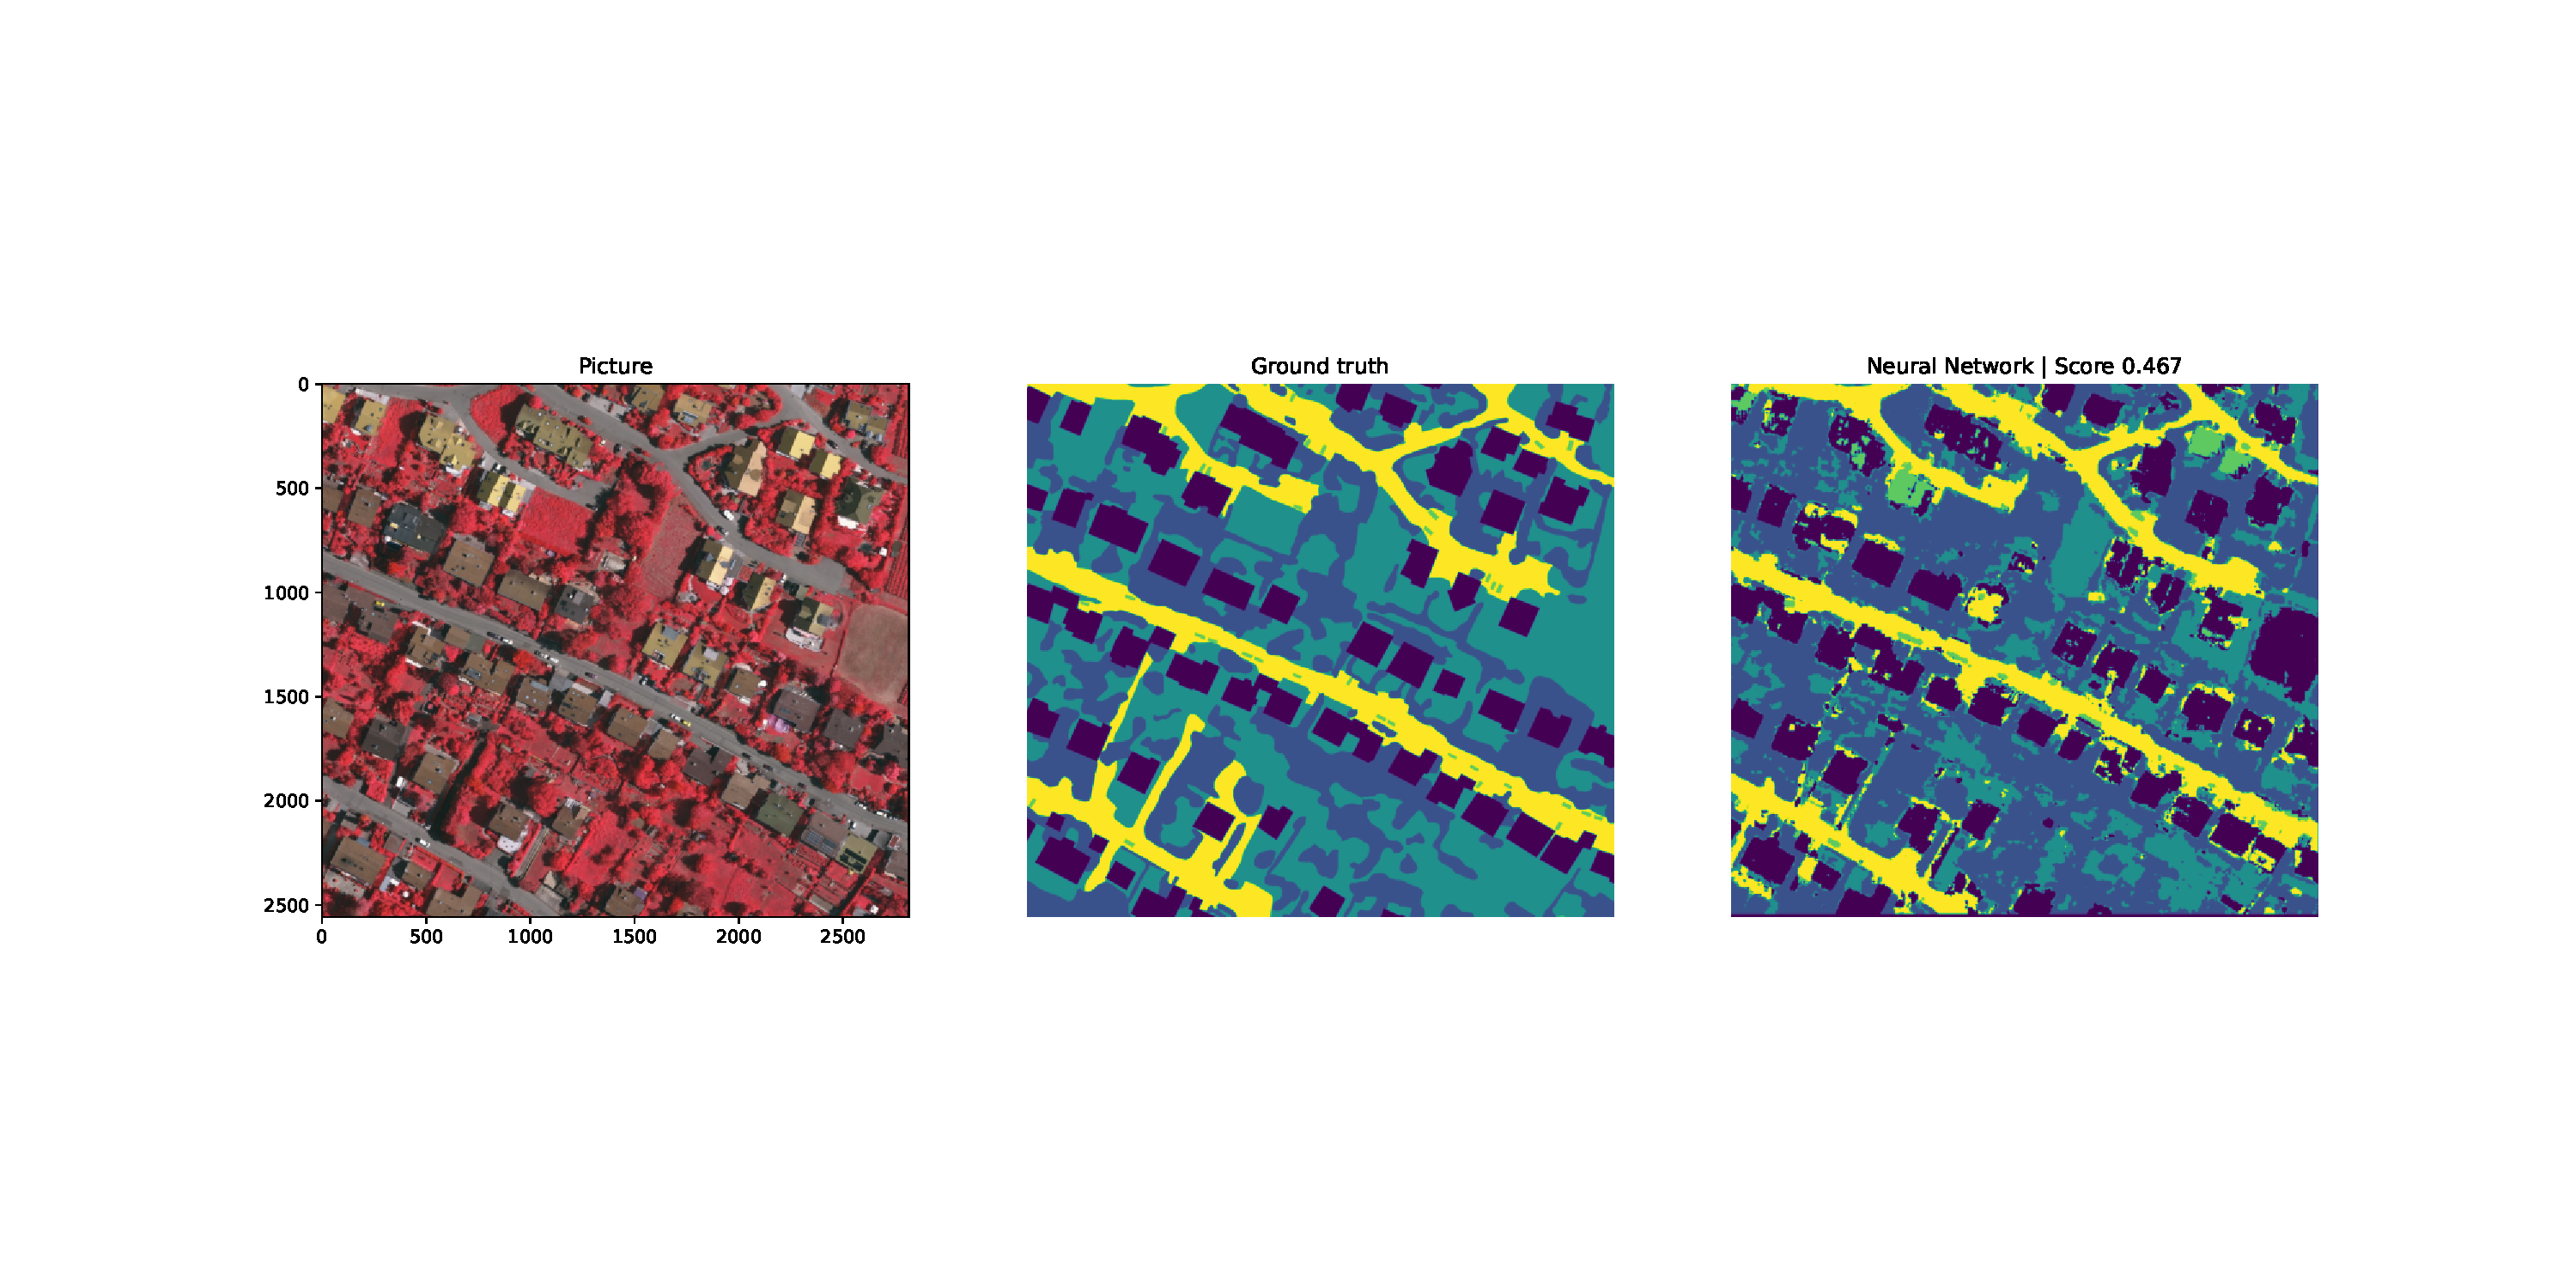
\includegraphics[width=\textwidth]{images/Patch32_scratch_test.pdf}
    \caption{test results}
    \label{fig:q2a_test}
  \end{subfigure}
  \caption{Results of predictions for item \ref{item:2a}}
  \label{fig:q2a_results}
\end{figure}

\subsection{Item \ref{item:2b}}

\lipsum[1]

\begin{figure}[htpb]
  \centering
  \begin{subfigure}[b]{0.32\textwidth}
      \centering
      
\includegraphics[width=\textwidth]{images/Patch64_scratch_loss.pdf}
      \caption{Loss evolution}
      \label{fig:q2b_loss}
  \end{subfigure}
  \hfill
  \begin{subfigure}[b]{0.32\textwidth}
    \centering
    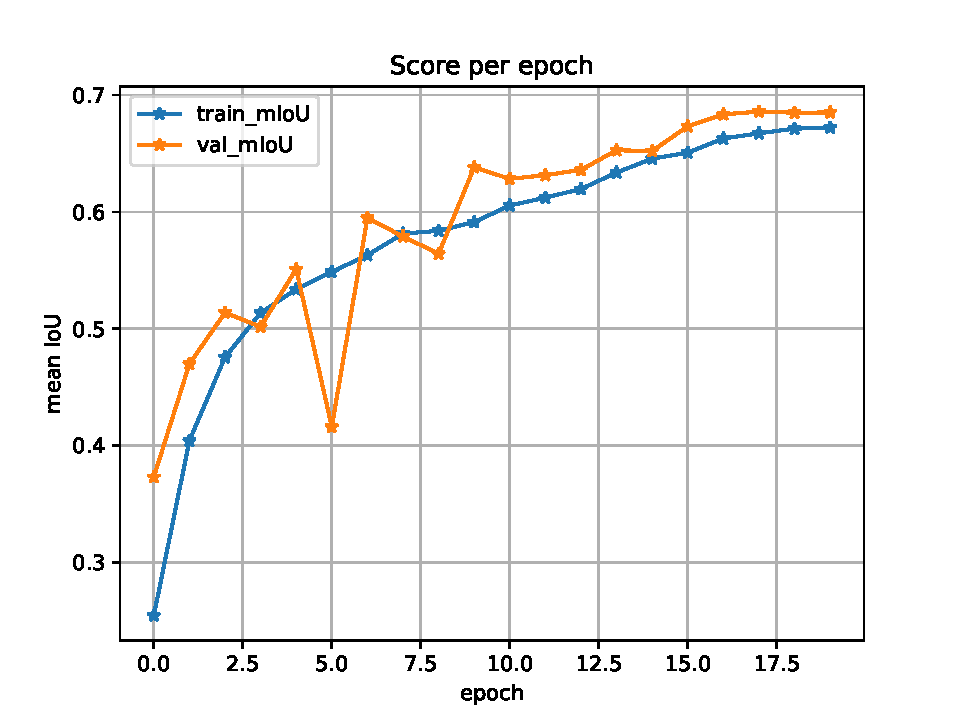
\includegraphics[width=\textwidth]{images/Patch64_scratch_score.pdf}
    \caption{Score evolution}
    \label{fig:q2b_score}
  \end{subfigure}
  \hfill
  \begin{subfigure}[b]{0.32\textwidth}
      \centering
      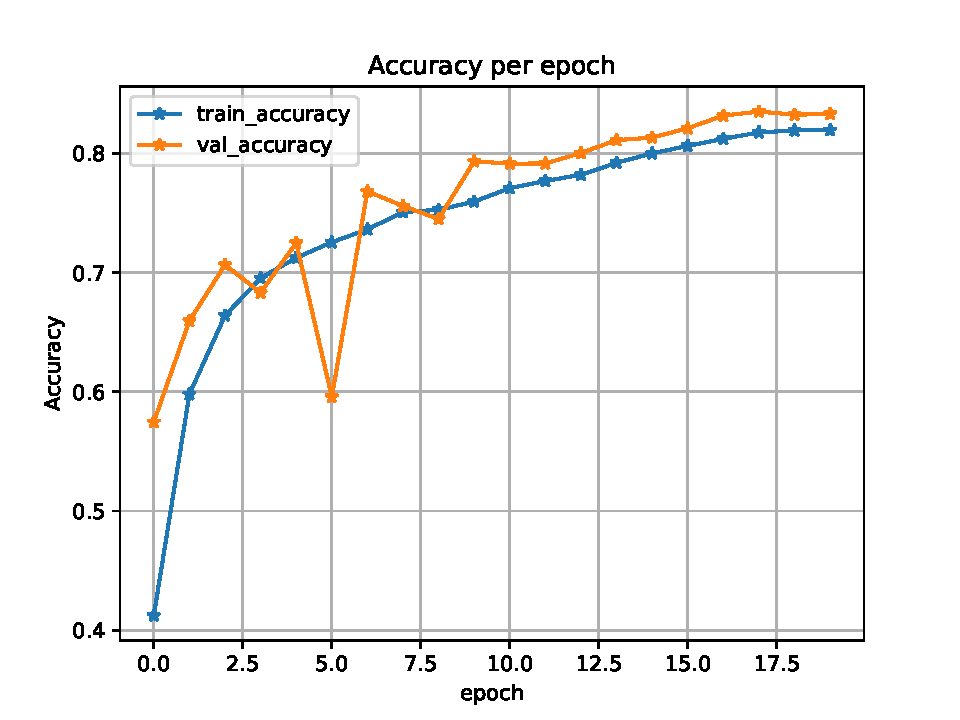
\includegraphics[width=\textwidth]{images/Patch64_scratch_acc.pdf}
      \caption{Accuracy evolution}
      \label{fig:q2b_acc}
  \end{subfigure}
  \caption{Metrics evolution during training for item \ref{item:2b}}
  \label{fig:q2b_metrics}
\end{figure}

\begin{figure}[htpb]
  \centering
  \begin{subfigure}[b]{1.0\textwidth}
      \centering
      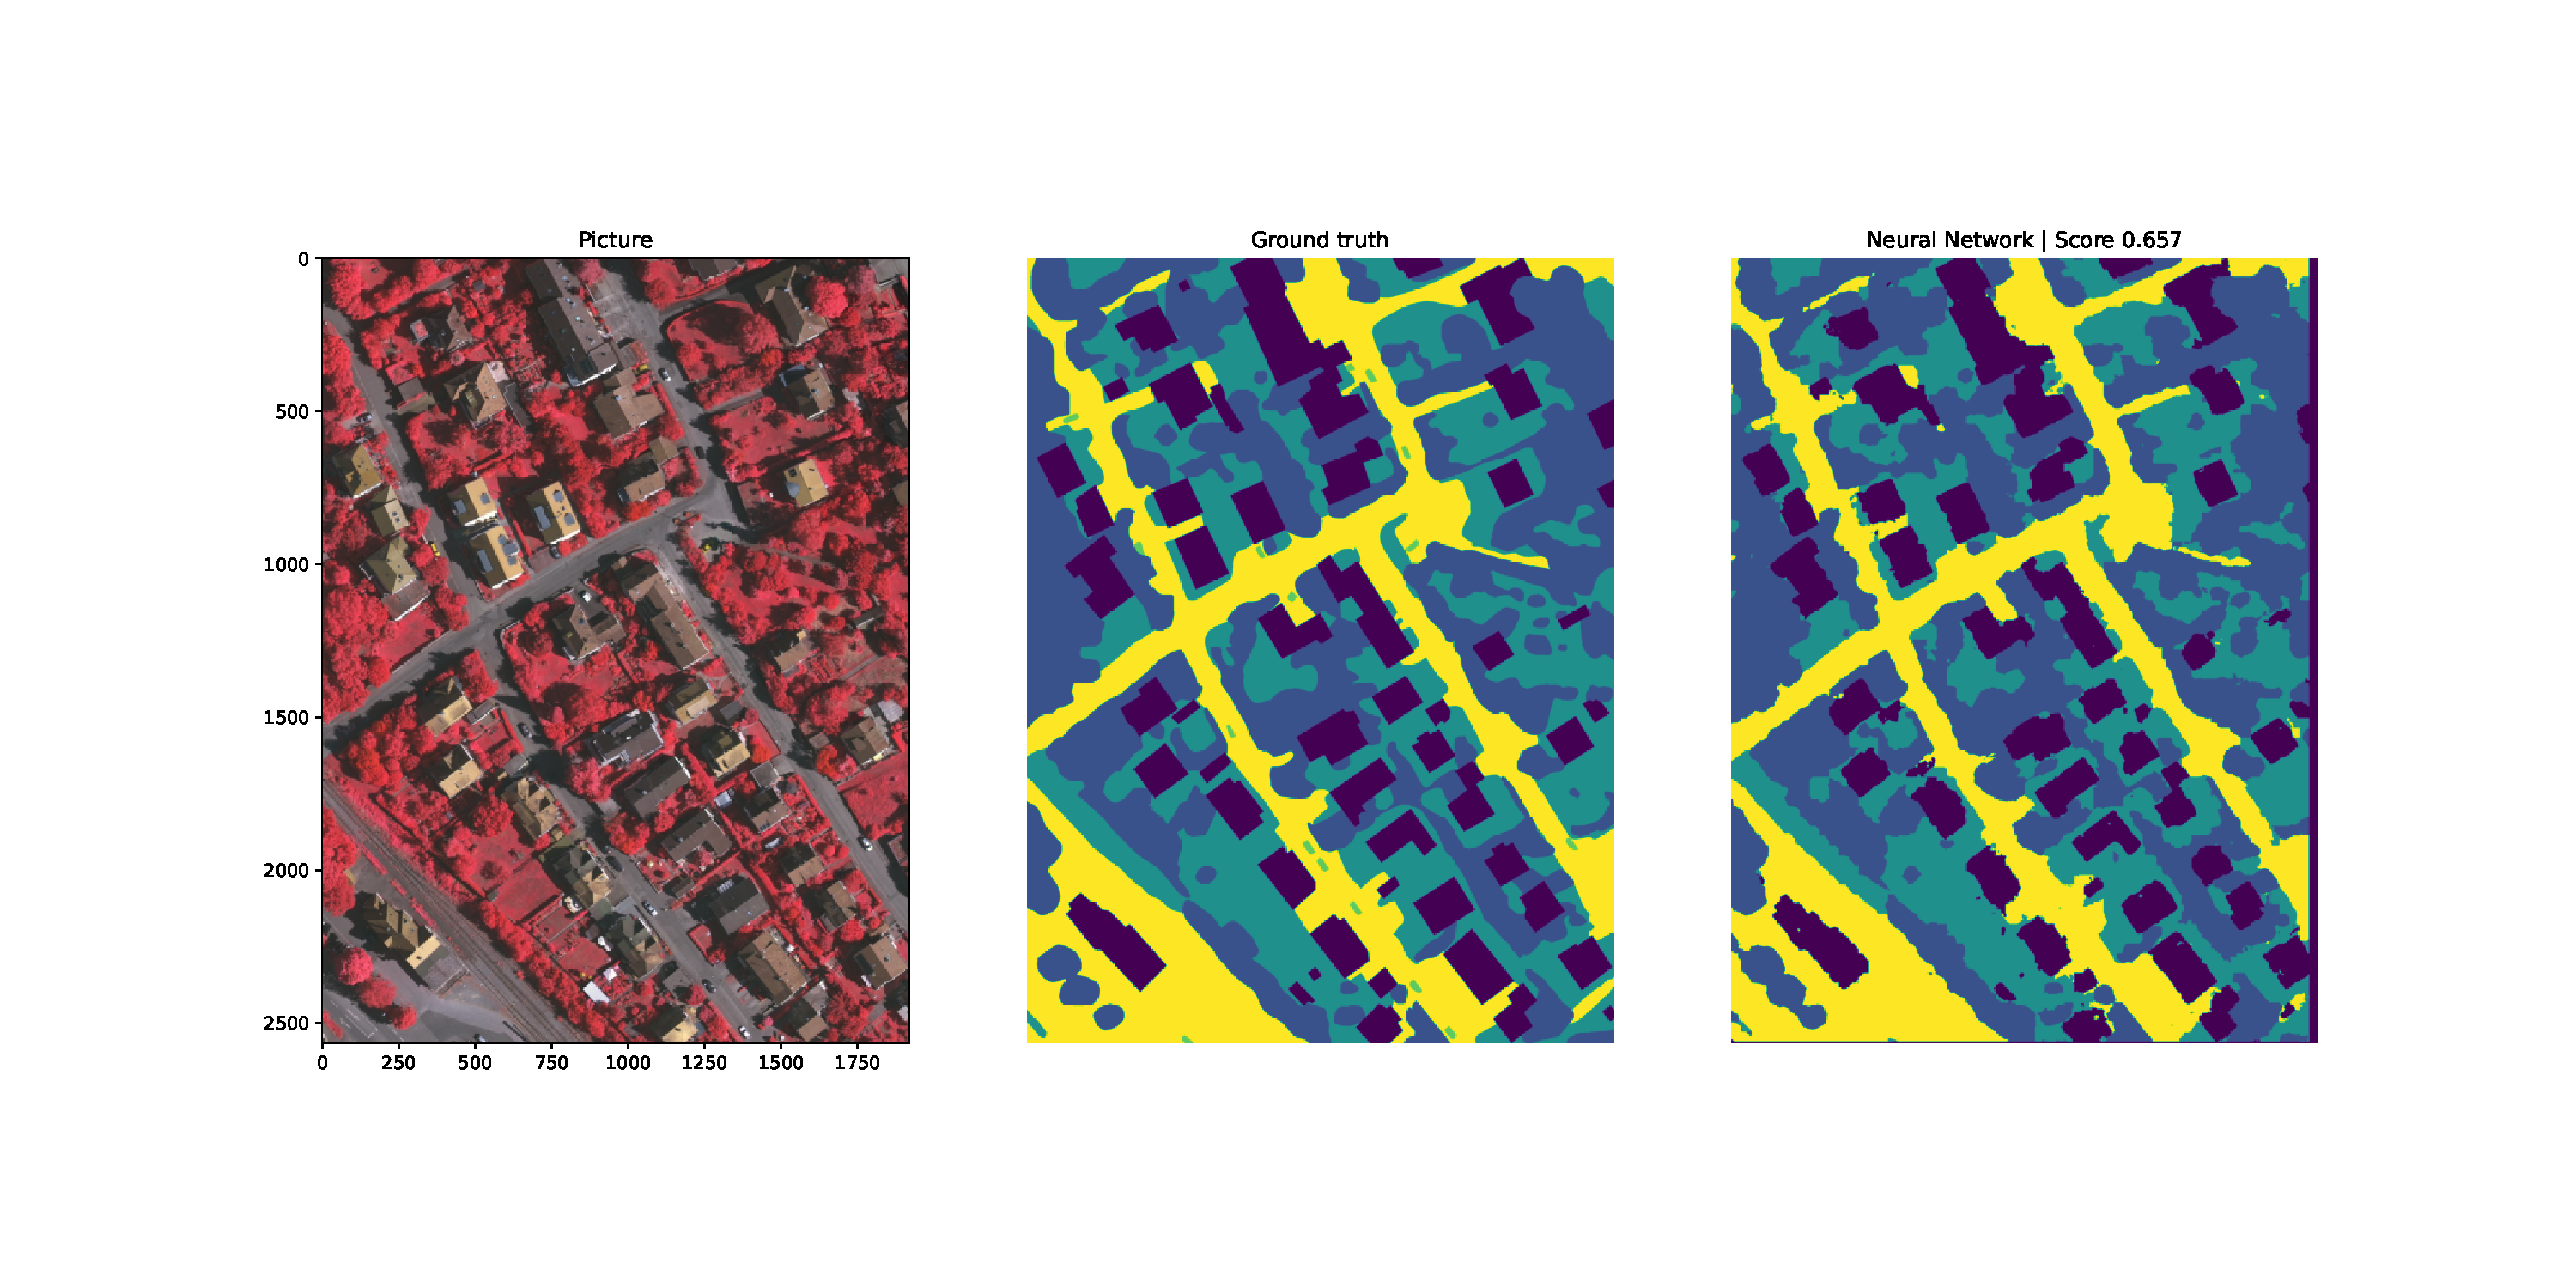
\includegraphics[width=\textwidth]{images/Patch64_scratch_train.pdf}
      \caption{Train results}
      \label{fig:q2b_train}
  \end{subfigure}
  \hfill
  \begin{subfigure}[b]{1.0\textwidth}
    \centering
    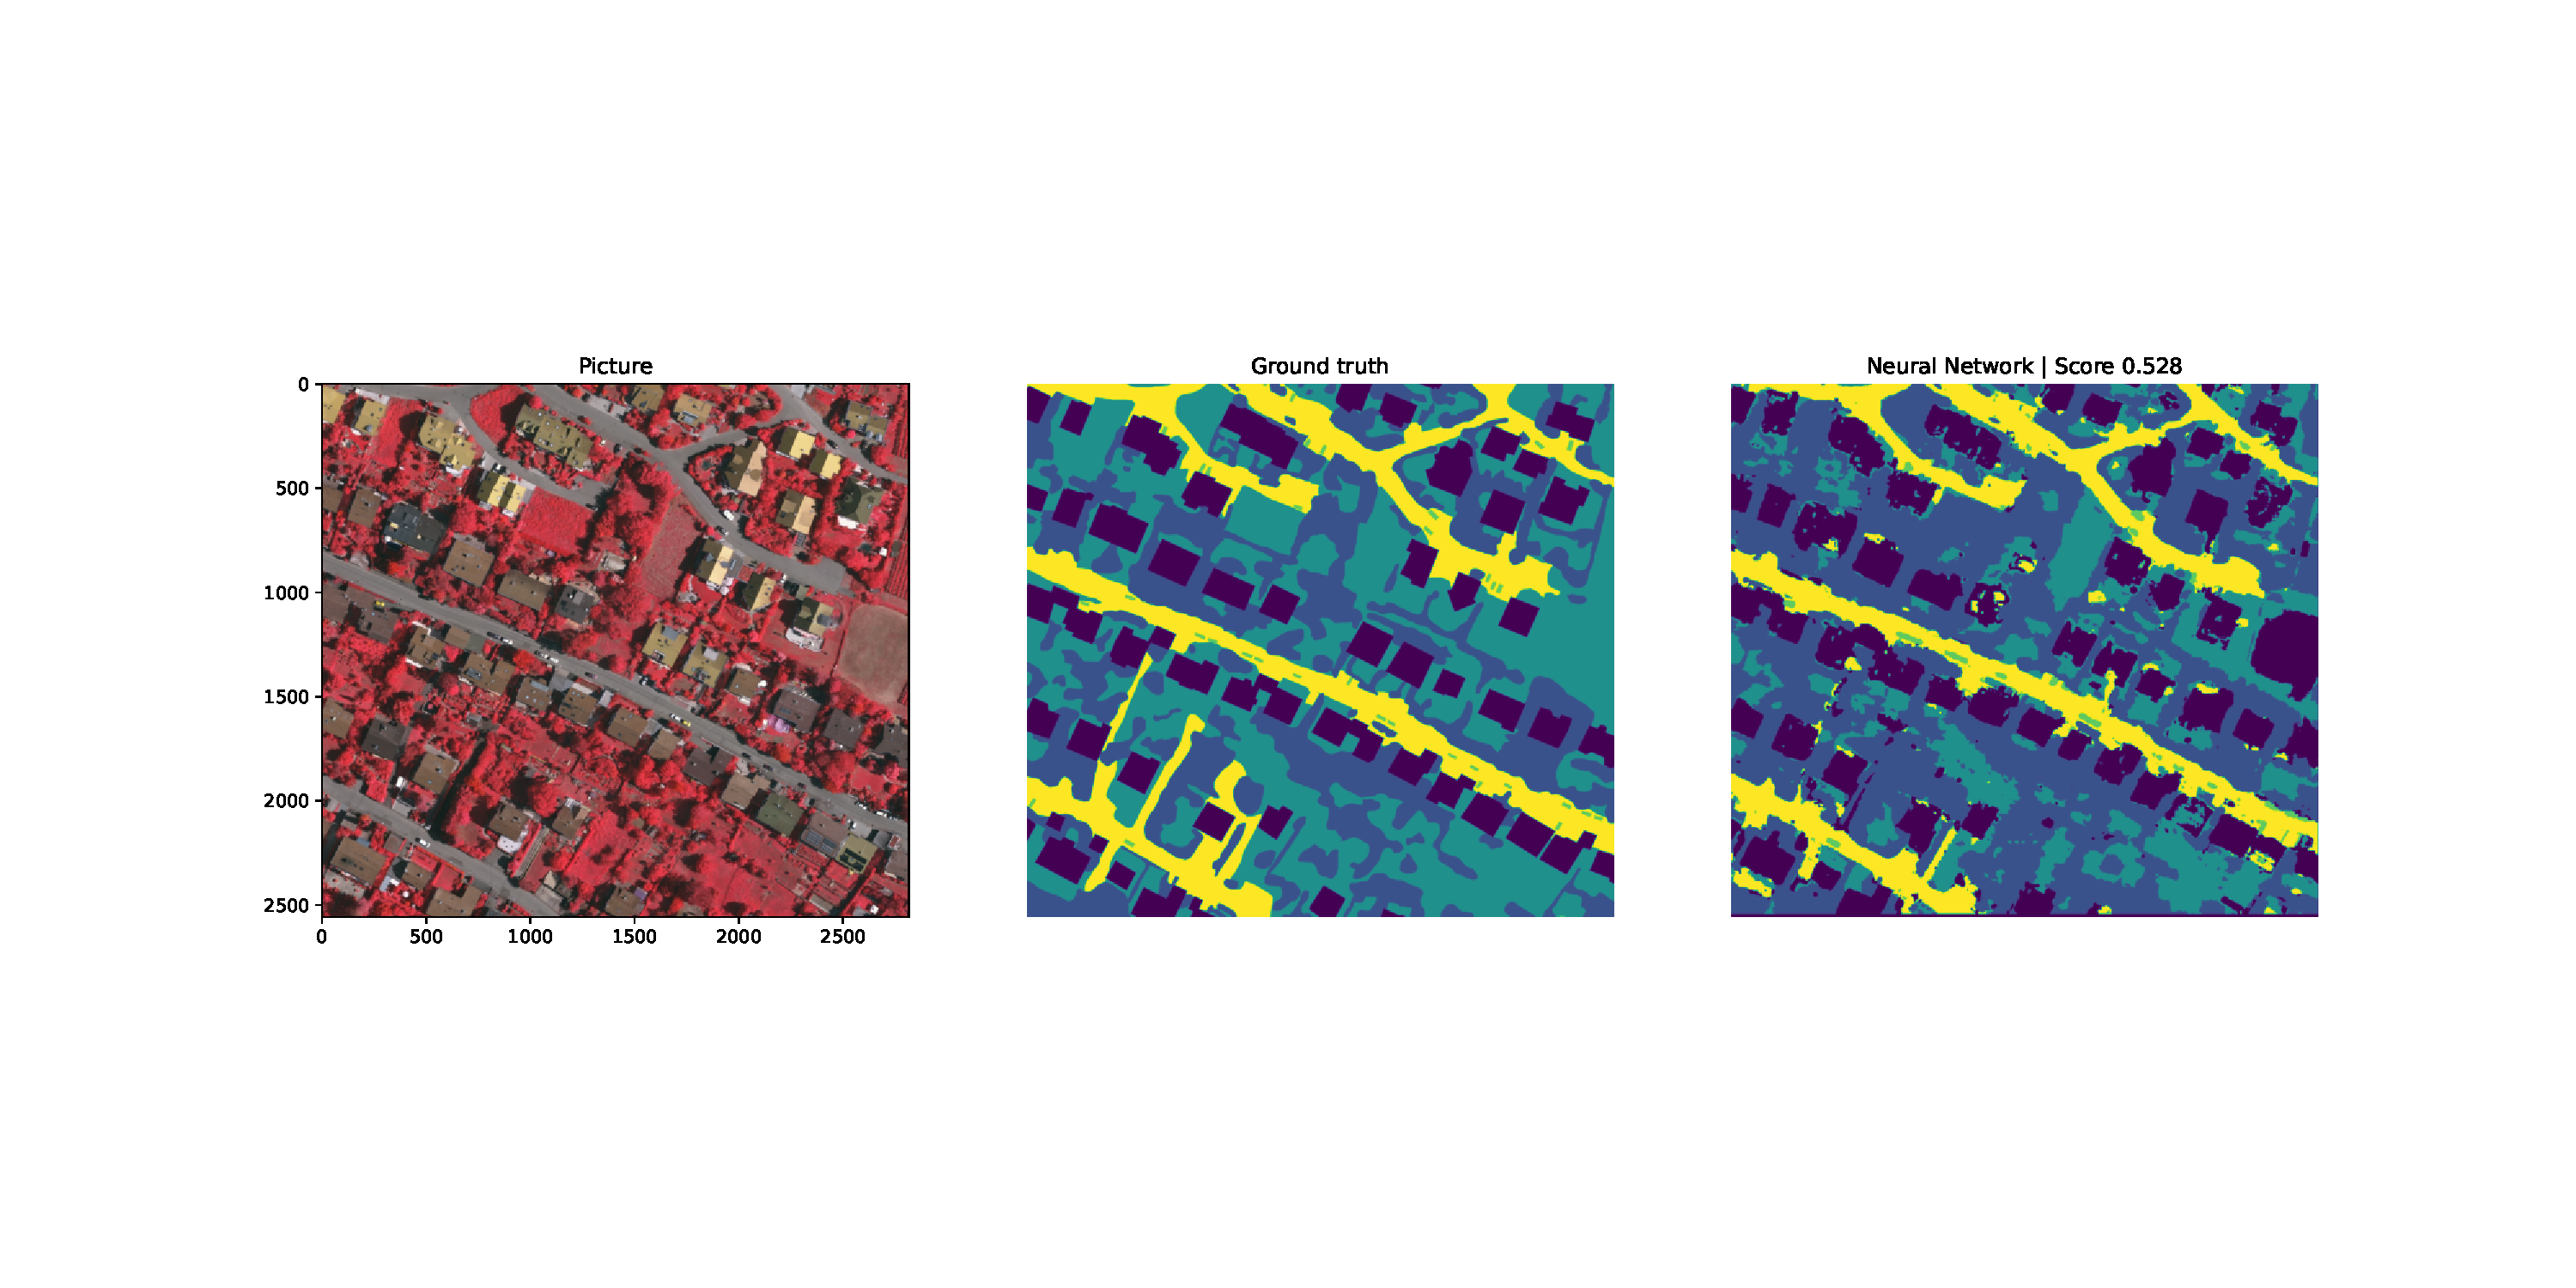
\includegraphics[width=\textwidth]{images/Patch64_scratch_test.pdf}
    \caption{test results}
    \label{fig:q2b_test}
  \end{subfigure}
  \caption{Results of predictions for item \ref{item:2b}}
  \label{fig:q2b_results}
\end{figure}

\subsection{Item \ref{item:2c}}

\lipsum[1]

\begin{figure}[htpb]
  \centering
  \begin{subfigure}[b]{0.32\textwidth}
      \centering
      
\includegraphics[width=\textwidth]{images/Patch128_scratch_loss.pdf}
      \caption{Loss evolution}
      \label{fig:q2c_loss}
  \end{subfigure}
  \hfill
  \begin{subfigure}[b]{0.32\textwidth}
    \centering
    
\includegraphics[width=\textwidth]{images/Patch128_scratch_score.pdf}
    \caption{Score evolution}
    \label{fig:q2c_score}
  \end{subfigure}
  \hfill
  \begin{subfigure}[b]{0.32\textwidth}
      \centering
      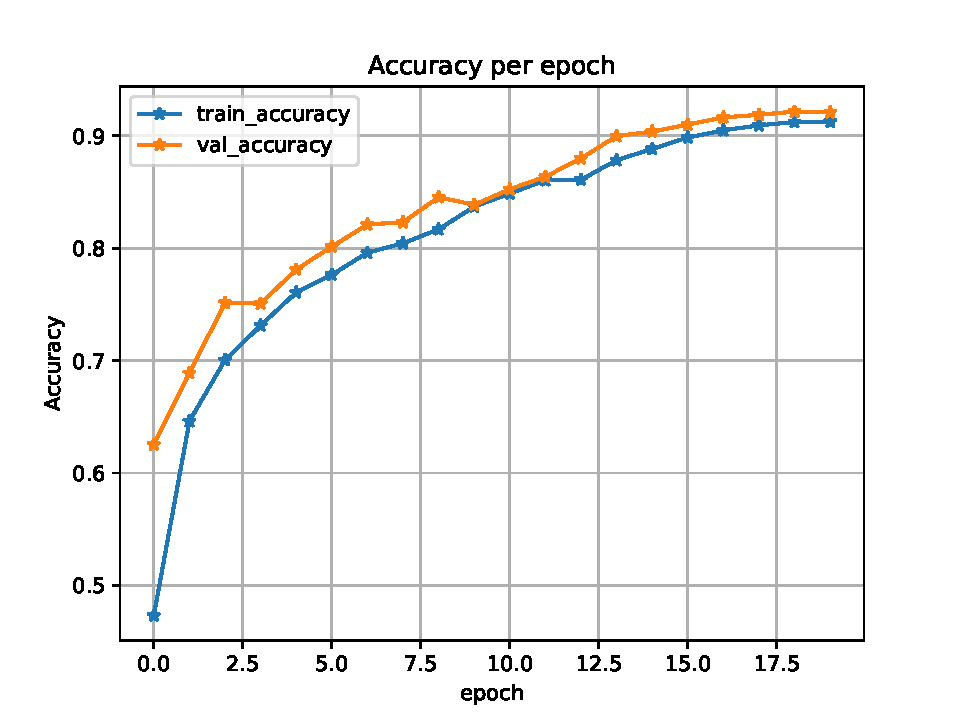
\includegraphics[width=\textwidth]{images/Patch128_scratch_acc.pdf}
      \caption{Accuracy evolution}
      \label{fig:q2c_acc}
  \end{subfigure}
  \caption{Metrics evolution during training for item \ref{item:2c}}
  \label{fig:q2c_metrics}
\end{figure}

\begin{figure}[htpb]
  \centering
  \begin{subfigure}[b]{1.0\textwidth}
      \centering
      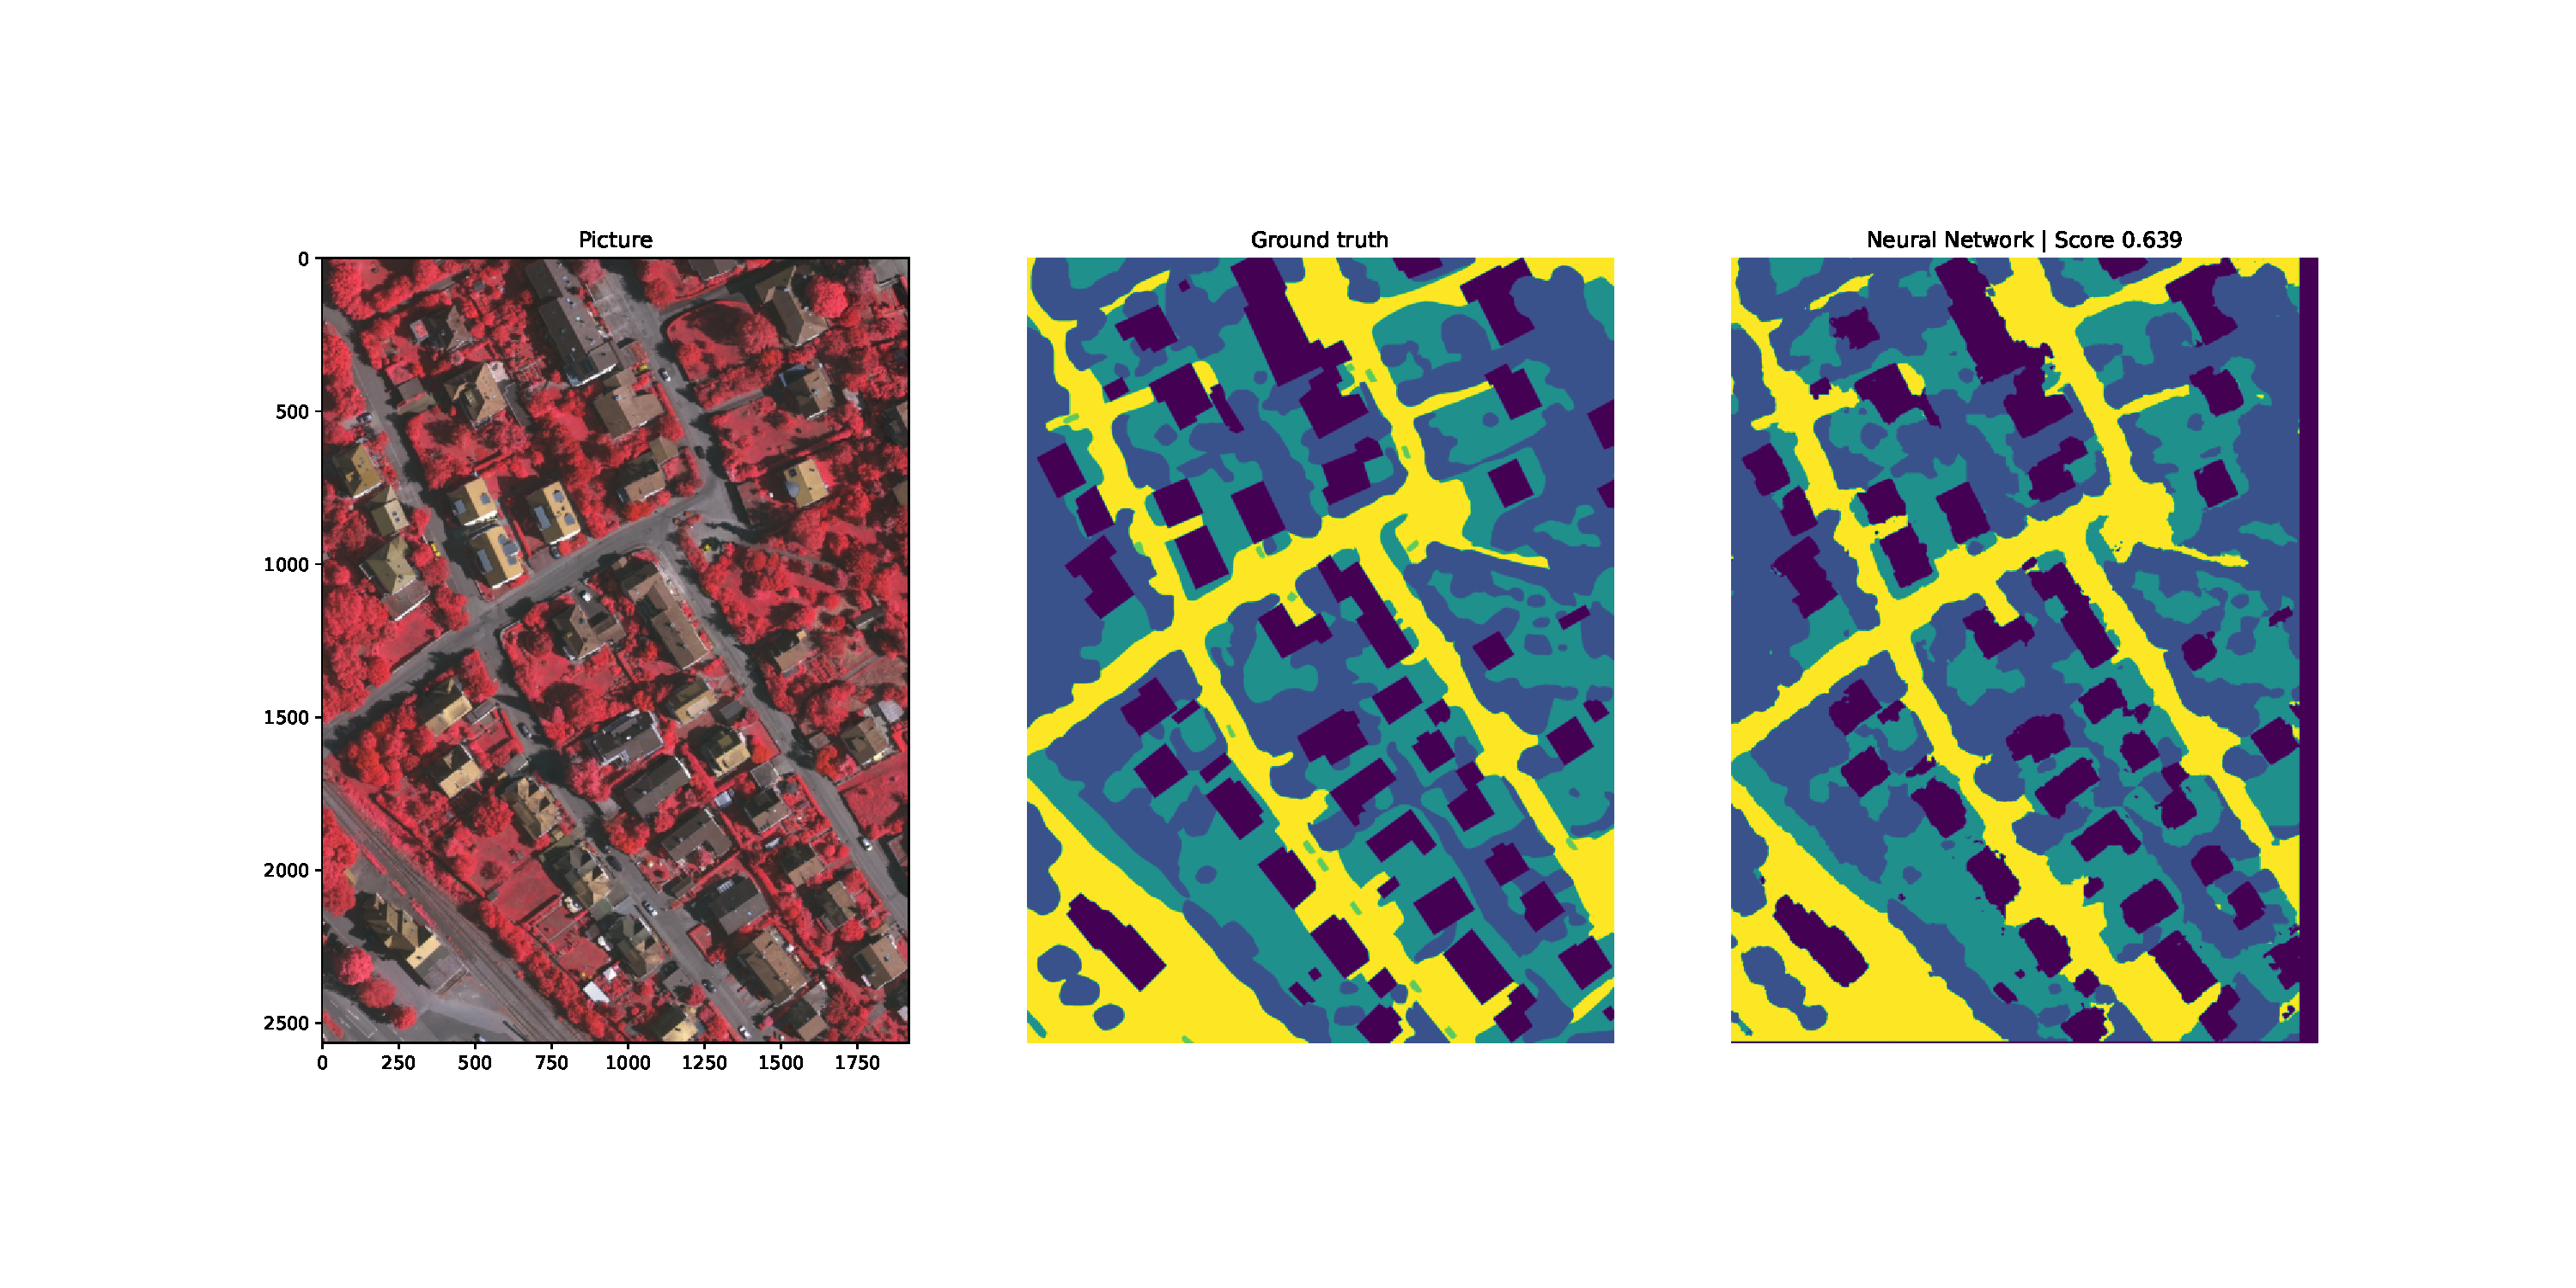
\includegraphics[width=\textwidth]{images/Patch128_scratch_train.pdf}
      \caption{Train results}
      \label{fig:q2c_train}
  \end{subfigure}
  \hfill
  \begin{subfigure}[b]{1.0\textwidth}
    \centering
    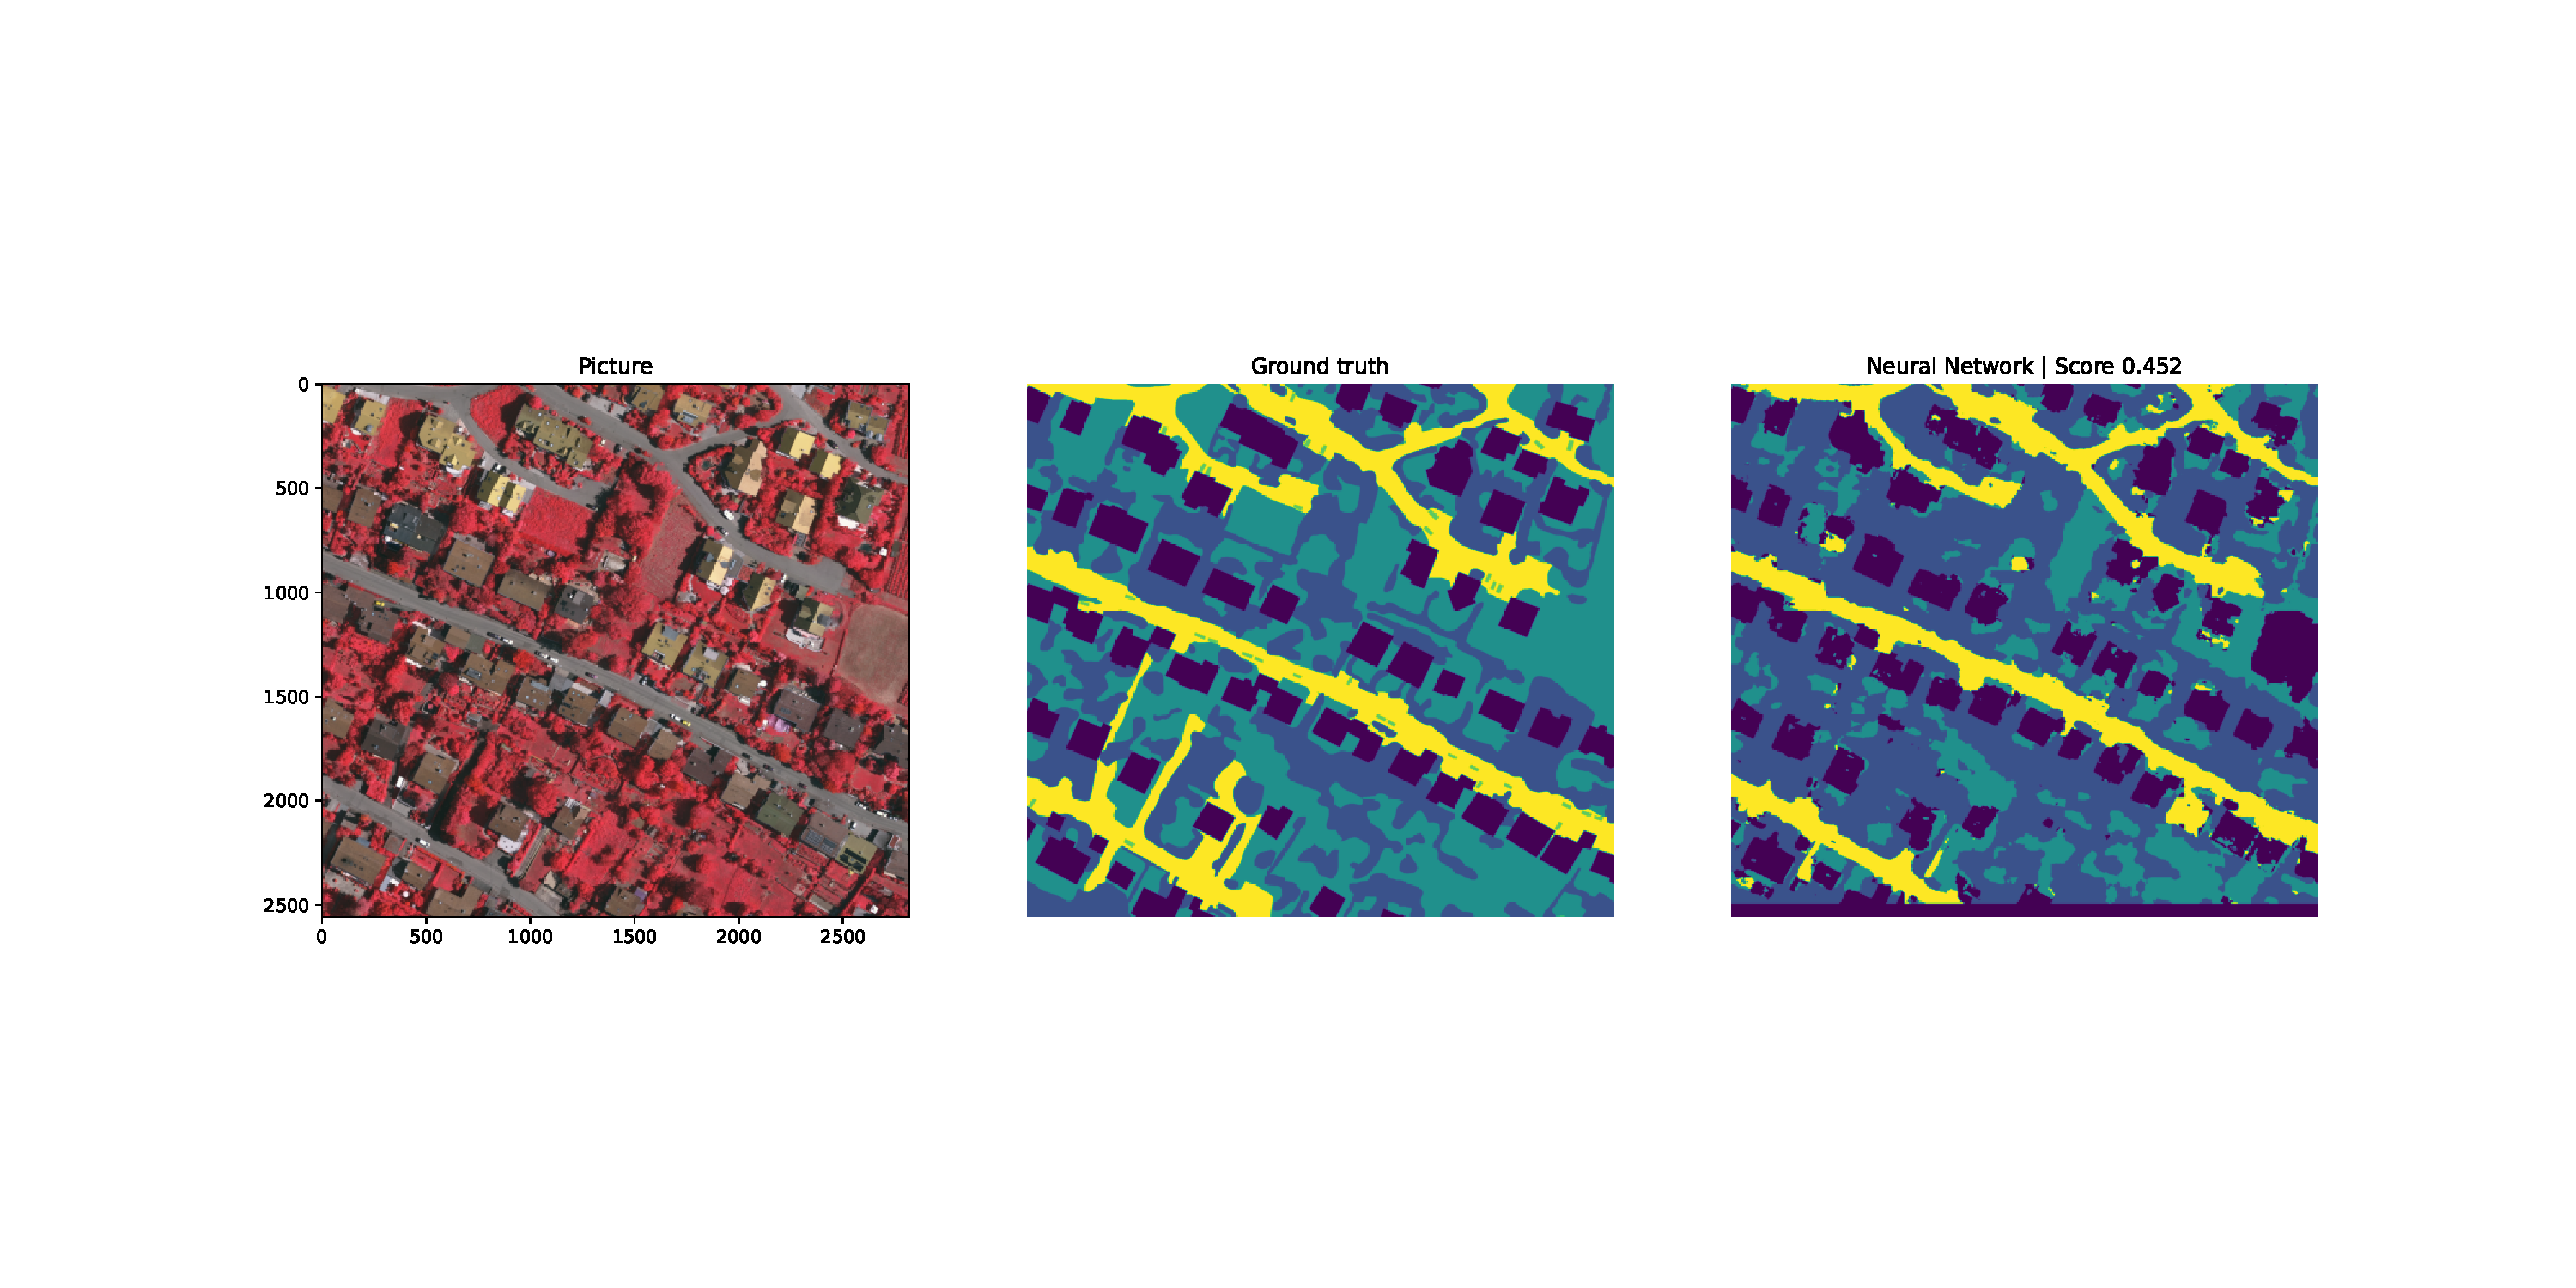
\includegraphics[width=\textwidth]{images/Patch128_scratch_test.pdf}
    \caption{test results}
    \label{fig:q2c_test}
  \end{subfigure}
  \caption{Results of predictions for item \ref{item:2c}}
  \label{fig:q2c_results}
\end{figure}

\subsection{Results Summary and Conclusions}

\begin{table}[htpb]
  \centering
  \begin{tabular}{l|c|c|c|c|c|c|c|}
    Exp             &	train acc	       & train loss	    & val acc  & val loss	 & test acc	 & test loss & training time \\
    \hline
    \ref{item:1a}   & 94.00\%          & 0.159551       & 94.74\%  & 0.174357  & 92.19\%   & 0.229864  & 14 min        \\
    \ref{item:1b}   & 87.43\%          & 0.329751       & 92.48\%  & 0.233386  & 85.94\%   & 0.390936  & 06 min        \\
    \ref{item:1c}   & 98.26\%          & 0.055598       & 98.50\%  & 0.056195  & 96.09\%   & 0.112185  & 03 min        \\
    \ref{item:2a}   & 95.84\%          & 0.121377       & 96.24\%  & 0.082859  & 91.41\%   & 0.176876  & 04 min        \\
    \ref{item:2b}   & 95.84\%          & 0.116910       & 98.50\%  & 0.076800  & 94.53\%   & 0.131344  & 11 min        \\
    \ref{item:2c}   & 95.84\%          & 0.116910       & 98.50\%  & 0.076800  & 94.53\%   & 0.131344  & 11 min        \\
    \hline
  \end{tabular}
  \caption{Results summary}
  \label{tab:results_summ}
\end{table}






%%%%%%%%%%%%%%%%%%%%%%%%%%%%%%%%%%%%%%%%%%%%%%%%%%%

\bibliographystyle{apalike}
\bibliography{export}

\end{document}